% Same-family audit draft; uncompiled and not a promoted reader edition.
% All legacy source/PDF pins remain at their original paths.
\documentclass[11pt]{article}
\usepackage[margin=1in]{geometry}
\usepackage{amsmath,amssymb,amsthm,booktabs,longtable,array}
\usepackage[T1]{fontenc}
\usepackage{hyperref}
\usepackage{tikz}
\usetikzlibrary{positioning,arrows.meta}
\setlength{\emergencystretch}{3em}
\newtheorem{theorem}{Theorem}
\newtheorem{lemma}[theorem]{Lemma}
\newtheorem{proposition}[theorem]{Proposition}
\newtheorem{corollary}[theorem]{Corollary}
\theoremstyle{remark}\newtheorem{remark}[theorem]{Remark}
\newcommand{\HH}{\mathbb H}
\newcommand{\QQ}{\mathbb Q}
\newcommand{\Dfive}{\mathcal D_5}
\newcommand{\cert}[1]{\nolinkurl{#1}}
\newcommand{\act}{\mathrm{act}}
\newcommand{\up}{\mathrm{up}}
\title{Corner payments and a dimension bound of 57\\
for finite-volume hyperbolic Coxeter polytopes}
\author{Coxeter Polytopes Frontier Project}
\date{24 October 2026; audit consolidation draft}
\begin{document}
\maketitle
\begin{abstract}
We prove a dimension bound of57 for finite-sided, finite-volume real
hyperbolic Coxeter polytopes. The argument assigns nonnegative weights
to corners of two-dimensional faces. Triangles and quadrilaterals require
enough total weight, while the finite and affine Coxeter diagrams at a
vertex limit how much weight can be spent there. A global incidence
inequality makes these requirements incompatible in dimension 58.
The finite-vertex upper bound is exactly 377, the curvature coefficient;
ideal vertices retain surplus at least 36, and the two global extrema
supply a further correction 4205. Exact finite certificates support the
local rule and the vertex estimates. We describe their algorithms and
the distinction between geometric coverage and arithmetic verification.
The treatment includes nonsimple ideal vertices, whose links are products
of simplices. A separate appendix proves the higher-dimensional exclusion,
including the unbounded range, without assuming that a facet is Coxeter.
\end{abstract}

\section{Statement and proof architecture}
\begin{theorem}\label{thm:main}
Every finite-sided, finite-volume real hyperbolic Coxeter polytope has
dimension at most 57.
\end{theorem}
No arithmeticity, compactness, simple-cusp or facet-count hypothesis is
imposed. The theorem belongs to the combinatorial approach to dimension
bounds developed by Vinberg, Prokhorov and Khovanskii: small faces
force local contributions that a high-dimensional vertex cannot
accommodate \cite{Prokhorov,Khovanskii}. The largest presently known
dimension of a finite-volume example is 21; Borcherds constructs an
arithmetic reflection group in that dimension \cite{Borcherds}.
Thus the present bound still leaves a substantial existence gap.

This is a computer-assisted argument. The exact endpoint is
\cert{fresh_d13_context_dimension57_20261018}; its recursive source
manifest identifies the immutable proof atlas.

The main argument excludes dimension58. Appendices~\ref{app:tail}
and~\ref{app:narrow-tail} treat every higher dimension: first by a finite
set of payment families, and then by an all-rank narrow-facet argument.
We do not infer this tail from the single excluded dimension, or pass
to a facet whose angles have not been proved Coxeter. The marked local
rules and their exact arithmetic certificates are internal parts of
the argument, not additional published assumptions.

For a two-face$F$ with$s(F)$ sides, write
\[
 \Dfive(P)=\sum_F(5-s(F)).
\]
A simultaneous nonnegative corner rule paying at least 2 on each triangle
and 1 on each quadrilateral gives an upper bound for$\Dfive$. The final
rule has finite-vertex charge at most 377. At an ideal vertex its actual
charge$C_{\act}$ satisfies$\kappa-C_{\act}\ge36$, where$\kappa$ is the
link shape curvature. The global lower bound is
\[
 \Dfive\ge377v_f+\sum_{v\text{ ideal}}\kappa(v)+4205.
\]
The contradiction is therefore
\[
 0\ge4205+36v_i>0.
\]
The remainder proves the local and arithmetic interfaces that make this
subtraction valid.

\subsection{The common counting argument}

An angle in this paper is a corner $(v,F)$ of an actual two-face.
A payment is a nonnegative weight $w(v,F)$. Write
$C(v)=\sum_{F\ni v}w(v,F)$ for its total charge at a vertex.
The elementary local-to-global step is worth stating independently
of the particular rule and of the certificate files.

\begin{lemma}[Payment comparison]\label{lem:payment-comparison}
Suppose every triangular face receives total payment at least 2
and every quadrilateral receives at least 1. Then
\[
 \Dfive(P)\le\sum_v C(v).
\]
More generally, suppose an incidence argument gives
\[
 \Dfive(P)\ge Bv_f+\sum_{v\text{ ideal}}\kappa(v)+\Delta,
 \qquad\Delta>0,
\]
while a simultaneous payment rule has $C(v)\le B$ at every finite
vertex and $C(v)\le\kappa(v)-\varepsilon$ at every ideal vertex,
where $\varepsilon\ge0$. These hypotheses are inconsistent.
\end{lemma}
\begin{proof}
A face with $s$ sides needs payment at least $5-s$. This is2
for a triangle and 1 for a quadrilateral. For $s\ge5$ it follows
from nonnegativity. Sum over faces and then over their corners.
Combining the resulting upper bound with the proposed lower bound
gives $0\ge\Delta+\varepsilon v_i>0$.
\end{proof}

The geometry enters in choosing a rule that works at every actual
face. The computation enters after that reduction, when the possible
vertex diagrams and their contextual costs have been specified.
The same corner may not be spent twice merely because two local
arguments could have used it: all priorities and compensations must
belong to one simultaneous rule.
Appendix~\ref{app:weights} gives that rule explicitly, as a function
of a marked whole vertex diagram. For the preliminary finite count
we use the same tables with the stated $B_{13}$ endpoint restored
and without the final three rank-15-guarded changes. We call this
preliminary function the preceding rule below.

The proof first separates into finite and ideal vertices. At a finite
vertex we maximize the rule over spherical forests of total rank 58.
At an ideal vertex we bound each affine factor, multiply by its
actual corner-fiber multiplicity, and compare with the curvature of
the product link. These branches reunite in the payment comparison.
The final changes to the rule use whole components: a visible path
inside a larger component does not carry the same contextual bonus.
Figure~\ref{fig:proof-branches} records this division.

\begin{figure}[t]
\centering
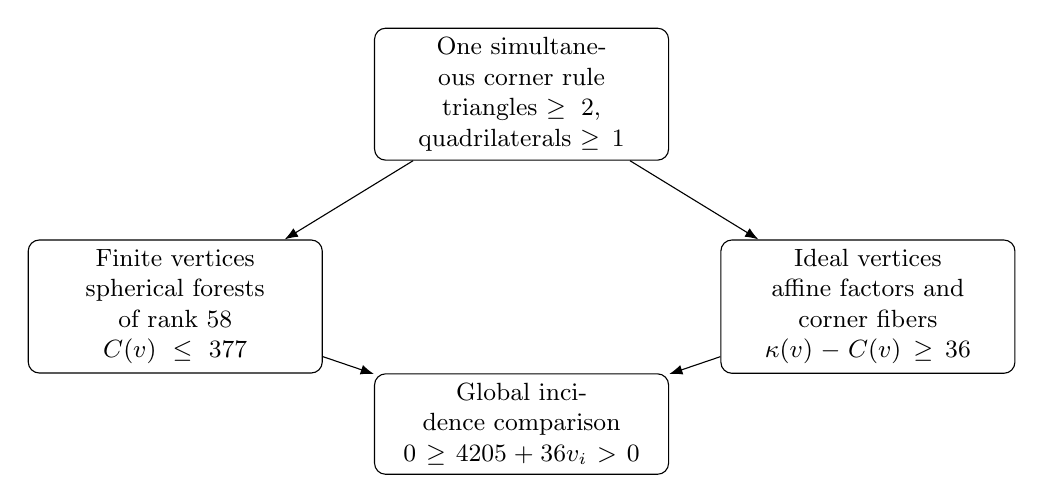
\begin{tikzpicture}[>=Latex,font=\small,
 box/.style={draw,rounded corners,align=center,text width=3.5cm,
 minimum height=1.1cm},node distance=1cm and .65cm]
 \node[box] (local) {One simultaneous corner rule\\
 triangles $\ge2$, quadrilaterals $\ge1$};
 \node[box,below left=of local] (finite) {Finite vertices\\
 spherical forests of rank 58\\$C(v)\le377$};
 \node[box,below right=of local] (ideal) {Ideal vertices\\
 affine factors and corner fibers\\$\kappa(v)-C(v)\ge36$};
 \node[box,below=2.7cm of local] (global) {Global incidence comparison\\
 $0\ge4205+36v_i>0$};
 \draw[->] (local)--(finite);
 \draw[->] (local)--(ideal);
 \draw[->] (finite)--(global);
 \draw[->] (ideal)--(global);
\end{tikzpicture}
\caption{The common geometric rule is established before the finite
and ideal arithmetic separate. The strict correction4205 comes from
the two extrema of a generic linear function on the polytope.}
\label{fig:proof-branches}
\end{figure}

\section{Actual corners, whole components and the previous finite count}
\label{sec:finite-interface}
We use outward norm-two roots, with diagonal Gram entries2 and
nonpositive off-diagonal entries. At an actual two-face in dimension$n$,
the supporting white roots form a positive-definite rank$n-2$ diagram.
White roots together with one black side give a strictly positive-definite
edge diagram; adjacent corners are positive semidefinite. A finite corner
has an elliptic forest of rank$n$.

These assertions refer to actual faces of the original chamber. We
record two elementary feasibility arguments that will also control
additional supporting roots. Let $p$ be a strict interior timelike
point. A positive-definite principal Gram matrix $B$ has nonpositive
off-diagonal entries and an entrywise nonnegative inverse. If
$b_i=-(p,e_i)>0$, then
\[
 q=p+\sum_i(B^{-1}b)_i e_i
\]
is orthogonal to the selected roots and has
$q^2=p^2-b^TB^{-1}b<0$. It is future pointing and strict against
every other chamber wall. Thus a positive principal set has an
actual finite common point, rather than merely a formal Gram model.

An irreducible affine principal set has a positive kernel vector
$(u_i)$. Its root combination $\nu=\sum_i u_i e_i$ is null and
nonzero, since $(p,\nu)<0$. It is feasible against every chamber
wall. Its projective point is an ideal vertex: an ideal-sphere point
is extreme in the closed Klein ball and hence in the chamber.
The affine diagram is a whole factor of that cusp, because every
proper principal subdiagram of an irreducible affine diagram is
positive definite. This is also the containment input
of~\cite[Section~1]{FeliksonTumarkin}.

\begin{lemma}[Opposite sides and minimal cores]\label{lem:opposite-cores}
For either opposite pair of sides of an actual quadrilateral, the
supporting whites and that pair form an indefinite principal set.
An inclusion-minimal indefinite subset contains both marked sides.
Its order is at most ten; if all proper principal subsets are
elliptic, its order is at most five.
\end{lemma}
\begin{proof}
A positive set would have an actual common finite point by the
projection argument. A positive-semidefinite singular set would
have a common ideal point by its affine kernel. Opposite closed
sides of a nondegenerate quadrilateral are disjoint, so neither is
possible. Deleting either marked side leaves a subset of an actual
finite edge diagram. Hence both marks lie in every minimal
indefinite subset. The published Lann\'er/quasi-Lann\'er order
bounds now apply; the classification through order ten
is~\cite{Chein}.
\end{proof}

Two such opposite cores cannot be disjoint and orthogonal, since
that would give two negative directions. Their overlap or a joining
path supplies an adjacent-side route. The local theorem must then
restore all the other supporting whites; an argument on the displayed
cores alone would not justify a whole-component payment.

A whole component is a connected component of the full actual corner
diagram, not merely of a displayed core. Presence conditions in a weight
refer only to such whole components. This distinction is essential when
additional supporting whites are restored.

\begin{lemma}[Two ways to seal a component]\label{lem:seals}
Let $G$ be the Gram matrix of an actual indefinite core.
\begin{enumerate}
\item A Gram-kernel vector $z$ of this core gives the actual zero
root relation $\sum_i z_i e_i=0$. Every further wall therefore
satisfies $\sum_i z_i(e,e_i)=0$.
\item Suppose $G$ is nonsingular, an added forest contacts it only
at a position $p$, and $(G^{-1})_{pp}=r>1$. If every connected
component of the added forest contacts $p$, its total rank is at
most $1/(r-1)$.
\end{enumerate}
\end{lemma}
\begin{proof}
The span of an indefinite core contains a timelike vector. The root
combination associated with a Gram-kernel vector is null and
orthogonal to that timelike vector. The perpendicular space is
positive definite, so the combination is zero. This differs from
the nonzero feasible null vector of an affine block.

For the second statement let $B$ be the positive Gram matrix of all
added supporting whites, including indirect tails, and let $u$ be
their contact column at $p$. Schur elimination and the one-negative-
direction condition give $B-r uu^T\succeq0$, whence
$u^TB^{-1}u\le1/r$.

For a connected square-two finite Coxeter Gram of rank $k$, every
inverse diagonal is at least $k/(k+1)$. This follows by induction:
delete the chosen node, let the remaining component ranks be $k_j$,
and use a contact of magnitude at least one into each component.
Inverse positivity gives Schur cost at least
$\sum_j k_j/(k_j+1)\ge(k-1)/k$. The resulting inverse diagonal
is at least $1/(2-(k-1)/k)=k/(k+1)$; the rank-one base is $1/2$.
For an added forest of total rank $M$ contacted in each component,
the same bound gives $u^TB^{-1}u\ge M/(M+1)$.
Thus $M/(M+1)\le1/r$, proving $M\le1/(r-1)$.
\end{proof}

The second argument takes all roots of the growing forest at once.
A bound on its immediate neighbors would leave indirect extensions
uncontrolled. For a radical seal, nonpositive contact signs and the
displayed zero relation restrict every further root; the local
short-path alternatives then force either a persistent payment or
orthogonality. An indirect extension has a first contacting root,
so this is the step that turns a core component into a whole one.

At an ideal vertex with affine factor ranks$r_i$, the link is
$\prod_i\Delta^{r_i}$, with$\sum r_i=n-1$. A marked pair in factor$i$
occurs in$\prod_{j\ne i}(r_j+1)$ actual corner fibers. Hence an affine
factor envelope$(r+1)c(r)$ gives
\begin{equation}\label{eq:envelope}
 C_{\act}\le C_{\up}=V\sum_i c(r_i),\qquad V=\prod_i(r_i+1).
\end{equation}
The factor-fiber theorem includes nonsimple ideal vertices. Whole affine
factors used locally are established by the positive kernel and actual
corner semidefiniteness, before applying this multiplicity.
Indeed an edge of the product link varies in just one simplex factor.
A fixed pair of its facet labels determines an edge in that factor
and an arbitrary vertex in every other factor. These are precisely
the $V/(r_i+1)$ fibers. The marked pair restores the varying affine
factor; all other factors appear with one node deleted. Summing an
unweighted copy of each affine table would miss this multiplicity.

\subsection{The finite forest algorithm}

For the finite calculation multiply charges by64. Its alphabet is
\[
 \{A_r:1\le r\le58\}\cup\{B_r:2\le r\le58\}
 \cup\{D_r:4\le r\le58\}
 \cup\{E_6,E_7,E_8,F_4,H_3,H_4,I_2^*\}.
\]
The rank-two symbol $I_2^*$ represents all remaining $I_2(m)$,
$m\ge5$, in the cost calculation. The local all-label theorem
gives their common relevant charge and interactions; this notation
is not a finite cutoff on $m$ or an identification of their metrics.
An admissible formal forest has multiplicities $m_T\ge0$ with
$\sum_T\operatorname{rank}(T)m_T=58$. Actual finite vertices are
among these forests. The calculation needs no converse realization
theorem.

The ordinary cost consists of a component table $b(T)$ and a
symmetric interaction table $j(T,U)$; context bonuses are separate.
In particular $j(T,T)$ concerns two distinct copies of $T$.
The cost is
\begin{align}\label{eq:forest-cost}
 C_{64}(m)&=\sum_T b(T)m_T+\sum_T j(T,T)\binom{m_T}{2}\notag\\
 &\quad+\sum_{T<U}j(T,U)m_Tm_U+\Psi(m).
\end{align}
The tables and the context function belong to the simultaneous
local rule. Their identification with actual corner charges is a
geometric obligation, separate from maximizing this expression.
Appendix~\ref{app:routing} supplies the actual-face coverage and
triangle arguments.
Appendix~\ref{app:finite-contexts} specifies the complete context
function and the finite refinement used in this calculation.

Fix all context-sensitive counts before the residual calculation.
After this split the residual alphabet $\mathcal U$ has positive
integer ranks $r(T)$ and additive integer weights $w(T)$, with no
remaining pair interaction. For a residual rank $R\le58$ define
\begin{equation}\label{eq:forest-dp}
 V(0)=0,\qquad
 V(s)=\max_{\substack{T\in\mathcal U, r(T)\le s\\
                         s-r(T)\text{ reachable}}}
       \{V(s-r(T))+w(T)\}\quad(1\le s\le R).
\end{equation}
An empty maximum is an unreachable state, not an ordinary integer.
Evaluate in increasing rank, recording a last item for each finite
maximum.

\begin{proposition}[Residual certificate]\label{prop:dp-certificate}
The algorithm~\eqref{eq:forest-dp} terminates and computes the exact
maximum over residual multisets. A saved table certifies the same
claim if it has base value zero, dominates every allowed last-item
transition, and has a tight last-item witness at every positive rank
carrying a finite stored value. At positive ranks, a state is
unreachable exactly when it has no reachable last-item predecessor;
rank zero is the reachable base.
\end{proposition}
\begin{proof}
There are at most 59 ranks and finitely many transitions at each
rank. Every predecessor has smaller rank. By induction, removing
one component from any nonempty multiset bounds its weight by one
of the candidates in~\eqref{eq:forest-dp}. Conversely, append the
chosen component to an attaining predecessor multiset. This proves
both inequalities and reachability. The same induction applies to
a saved table using all its transition inequalities and tight
witnesses at every stored finite value. Positive item ranks make
each tight predecessor smaller, so strong rank induction rules out
spurious finite entries. Following witnesses reaches zero after at
most 58 steps.
Checking only an attaining path would not bound omitted multisets.
\end{proof}

In the actual context split, fixed representative counts have
$\sum_{r=9}^{17}rc_r\le58$, with a separate $A_{12}/D_{12}$
split, fixed $A_{17}$, and $0\le k_5\le
\lfloor(58-\sum rc_r)/5\rfloor$. The residual ranks are
$1,2,3,4,6,7,8$ and 17 through 58. Expand every class that can exceed
377 into all actual-type fibers. Within each fiber fix the complete
$A_1,A_2$ counts. For the only remaining presence guard, split into
no $A_3$ or reserve one $A_3$ and allow further copies without
repeating its $D_{14}$ bonus. The two exceptional increasing families
are bounded separately, rather than omitted from the context cover.
All count ranges are bounded by rank 58. These facts prove termination
of the full context algorithm; the geometric domination theorem
establishes that its cover includes every actual forest.

\begin{proposition}[Computed finite interface]\label{prop:oldcount}
The preceding simultaneous rule in ambient 58 pays every triangle at
least2 and every quadrilateral at least 1. Every actual rank 58 finite
forest has charge at most 377 except precisely the following eight formal
forests: one$B_{13}$ or$D_{13}$ together with any multiset of three
$A_{15}$ or$D_{15}$ components. Each of those eight has charge378.
All ideal weights admit the envelope of Section~\ref{sec:ideal}.
\end{proposition}
\begin{proof}[Certificate and completeness argument]
The frozen coupled count starts from the complete 3298 fixed-vector/rank 5
cover, retaining fixed$A_{17}$ separately from residual$D_{17}$ and
separating the$A/B_{12}$ and$D_{12}$ interaction types. Simultaneous actual
base and cross-cost domination covers exceptional finite types and the
arbitrary-label rank-two family. Its two potentially increasing context
families are bounded separately:759 rows for the$A_1/D_5$ upgrade, and
539 rows for the$A_2/A_4$ guarded family, with all 14 costly rows refined
through 77 actual assignments. Both bounds are strictly below377.

The complementary complete 39 costly classes have748 fixed actual-type
fibers. All actual$A_1,A_2$ multiplicities are fixed explicitly. The
remaining$A_3$ presence guard is split into no$A_3$ and one reserved$A_3$;
the latter may contain more$A_3$ without multiplying the presence bonus.
All other context guards are fixed, and residual pair interactions vanish.
The1549 fresh residual tables certify every allowed last-item inequality,
unreachable rank and attaining predecessor. Induction on an item's removal
therefore proves their upper bounds for arbitrary residual multisets.
Reconstructing every winning forest verifies its full contextual cost.
All38 other classes are at most 377; the residual-zero rank 13-plus-three15
class gives exactly the eight listed forests. Their charge is$78+3(100)$.

The complete source, saved tables and separate replay are in
\cert{fresh_d17_a16_coupled_ambient58_frontier_20261018}. This proof
interface is not inferred from sampled maximizing forests. The written
universal local atlas is also required; the Bellman certificate alone does
not prove that its costs correspond to valid corner payments.
\end{proof}

A separate frozen$B_{13}$ endpoint theorem removes pair$(0,12)$, with no
new coupon. Its complete selected domain has no affected image, but that
absence alone is insufficient: two older affine-$B_{13}$ singleton routes
really consumed the endpoint unit. Their whole cores instead give distinct
already-unit$A_1/D_{12}$ short-leaf contributions. The other endpoint-like
pair$(1,12)$ needed by the current$D_{12}$ theorem is retained. Thus the
four$B_{13}$ forests in Proposition~\ref{prop:oldcount} drop to 377.

\section{The dimension-specific final local rule}
\begin{theorem}[Three-rank 15 transfer]\label{thm:local}
In ambient dimension 58, make these changes to the simultaneous rule:
\begin{enumerate}
\item In a whole finite$D_{13}$, give pairs$(0,11),(0,12)$ weight$1/2$
instead of1 only if its actual corner has three distinct whole unmarked
$A_{15}$ or$D_{15}$ components.
\item Add$1/2$ to whole$D_{28}$ pair$(0,12)$ only if its corner has two
such whole unmarked rank 15 components.
\item Add$1/2$ between an endpoint of whole$A_{12}$ and the long endpoint
of whole$D_{16}$ under the same two-component presence guard.
\end{enumerate}
All ideal weights and other finite weights remain. Every triangle still
pays at least 2 and every quadrilateral at least 1.
\end{theorem}
Witnesses are not counted with multiplicity. The negative guard uses
$13+3\cdot15=58$ ranks, so the corner has exactly those four components.
The two positive guards similarly force exactly$D_{28}+2\cdot15$ or
$A_{12}+D_{16}+2\cdot15$. The theorem is not asserted in larger ambient
dimensions.

\subsection{A general inverse bound for attached forests}
\begin{lemma}\label{lem:inverse}
For a connected positive-definite Coxeter Gram matrix$B$ of rank$k$,
with diagonal2 and every nonzero native magnitude at least 1,
$(B^{-1})_{ii}\ge k/(k+1)$ for every$i$. If a finite forest of total
rank$M$ has a nonnegative contact vector$u$ with at least one unit contact
in every component, then$u^tB^{-1}u\ge M/(M+1)$.
\end{lemma}
\begin{proof}
Inverse matrices of these positive-definite symmetric$Z$-matrices are
entrywise nonnegative. Delete the chosen root; let the remaining connected
components have ranks$k_j$. Every component has a contact with the root.
By induction and inverse positivity its contribution to the root's Schur
projection is at least$k_j/(k_j+1)$. Since
\[
 \sum_j\frac{k_j}{k_j+1}\ge\frac{\sum_jk_j}{1+\sum_jk_j}
 =\frac{k-1}{k},
\]
Schur complementation gives
$(B^{-1})_{ii}\ge(2-(k-1)/k)^{-1}=k/(k+1)$.
The rank-one base is$1/2$. Larger native magnitudes or multiple contacts
only increase the lower bound. Apply it in every contacted component of
a forest and use the same sum inequality to prove the second assertion.
\end{proof}

\subsection{Complete selected cases and arbitrary additional whites}
The fresh complete target domain contains801 patterns,862$D_{13}$ maps,
33 affected contexts and 76 affected pair maps. The physical cores have
norm-two roots; full Lorentz, white and all four edge signatures and actual
corner classifications are reconstructed exactly. The native-domain
completeness is inherited from the universal reduction, rather than
claimed from these records alone.

There are five proper completions. Their missing fork leaf is genuinely
new: old corner roots outside the displayed$A_{12}$ are orthogonal to it.
Its forced unit contact has inverse projection square6,12,30 or102,
exceeding2. Additional same-end contacts cannot lower the bound. Mixed-end
contacts give an independently paid short path. Thus these completions
are impossible.

Four radical cores, numbered1985,2378,2575,2581, seal the entire displayed
core. Indeed the whole selected$D_{13}$ forbids contacts on its nodes;
every remaining contact position has a nonzero radical coefficient. A new
white must pair to zero with the radical. Nonempty contacts therefore
meet both signs and give a retained adjacent-black shortcut of length at
most8. Otherwise all contacts vanish and the unmarked$A_4$ is whole.
It cannot coexist with the three rank 15 witnesses.

Twelve contexts similarly have a small displayed block with no permitted
new contact of projection at most 2. It is whole: any indirect extension
would have a first new root contacting it. The rank-capacity guard again
excludes it.

In the final twelve contexts the old small factor$K$ has rank$s=1,2,3$.
Its unique permitted contact position$p$ has core-inverse square
$r=4/3,3/2,2$, respectively. The native gap excludes magnitudes greater
than1; positive-end inverse bounds exclude two same-end contacts.
Four cases also permit an opposite contact position$q$, with
$J_{pp}=J_{qq}=4/3$ and$J_{pq}=-4/3$. Two new roots using$p,q$ have residual
squares$2/3$, so their full product is at most$-4/3+2/3=-2/3$. Their
forced native bond supplies the retained short path. Thus, without that
escape, all new whites in a growing$K$ component contact the old core
only at$p$; some may be orthogonal to it.

Let$Y$ contain all new whites in this whole component, including every
indirect tail, and let$M$ be its rank. Every component of$Y$ contacts$K$.
With contact vector$u$, the full Lorentz condition gives the positive
semidefinite residual Schur matrix
\[
 G_Y-r uu^t\succeq0,
 \qquad u^tG_Y^{-1}u\le1/r.
\]
Lemma~\ref{lem:inverse} implies$rM/(M+1)\le1$, hence
$M\le3,2,1$ respectively. In all cases the whole$K$ component has rank
at most 4, contradicting the guard. This controls arbitrary supporting
whites, not just immediate neighboring roots.

\subsection{The universal affine-D12 consumer}
The old opposite-fork-leaf affine-$D_{12}$ theorem genuinely used the
newly lowered whole finite$D_{13}$ unit. It must be repaired separately.
Number its affine factor$F$ of order13 with spine0 through 8, short leaves
9,10 at0 and 11,12 at8. Choose ideal marks$a=9,b=11$ and opposite black
roots$c,d$. Let$Z$ be the elliptic spectator forest, orthogonal to$F$,
and$x,y$ the nonnegative contacts of$c,d$ with$Z$.

An adjacent-black bond or a shared spectator neighbor is an independently
paid short path. Otherwise$x,y$ have disjoint supports. The complete
all-label end-profile reduction gives each end cost at most 8; a
nonextreme end has cost at most 4. The exact Schur identity is
\[
 \frac{\det S}{h^2k^2}
 =1-\frac{g_c+g_d}{12}
  +\frac1{12}(x/h-y/k)^tG_Z^{-1}(x/h-y/k).
\]
Its determinant vanishes at the actual four-black star.

If an end is nonextreme, equality forces costs8 and 4 and$x=y=0$.
A quiet root attached to the selected old leaf gives the retained whole
$A_1/D_{12}$ short-leaf unit. If it attaches to the mate, it gives whole
$D_{13}$. Without the new guard its unit is unchanged. With the guard,
$Z$ consists of exactly three orthogonal whole rank 15 factors.
The three nonextreme equality profiles give, at a distinct corner,
respectively a retained$A_1/D_{12}$ unit, an independent whole affine
$B_{13}$ priority, or a second guarded$D_{13}$ half. These exhaust24
physical cases. The current$B_{13}$ endpoint repair uses its$D_{12}$
cross unit, not a newly financed$D_{13}$ route; there is no circularity.

When both ends are extreme,$h=k=1/2$, and the determinant becomes
\begin{equation}\label{eq:energyone}
 (x-y)^tG_Z^{-1}(x-y)=1.
\end{equation}
The old two-nonempty-support theorem gives retained short paths or small
sealed alternatives. The changed$D_{13}$ output belongs to the arbitrary
one-sided branch, say$y=0$. The quiet corner excludes$c$ and retains$Z$
orthogonally. If its$D_{13}$ guard holds,$Z$ is exactly three whole
$A_{15}/D_{15}$ factors.

\begin{lemma}\label{lem:rank 15}
Under the strict edge conditions and disjoint-support hypothesis,
energy1 on three whole$A_{15}/D_{15}$ factors forces a single unit contact
at the long endpoint of one$D_{15}$, by one black root. The other two
factors have zero contact with both black roots.
\end{lemma}
\begin{proof}
For $A_{15}$ the inverse diagonal entries below2 occur only at nodes
0,1,13,14. They are $15/16$, $7/4$, $7/4$, and $15/16$, respectively.
Two native contacts give energy
at least 2 and violate strict edge positivity. The complete profiles are
simple contacts at these four nodes or doubled contacts at0,14. The next
native squared magnitude$(3+\sqrt5)/2$ is already excluded.
For$D_{15}$ only its long endpoint has inverse diagonal below2, equal
to 1, and only its simple contact fits.

Every allowed nonzero component energy is at least$15/16$; no$A_{15}$
profile has energy1. The finite exact inverse table also checks every
disjoint two-sided profile difference: all are at least$15/16$ and none
is1. Equal-node contacts are forbidden by disjoint support. Two active
components would have total at least$15/8>1$. Equation~\eqref{eq:energyone}
therefore forces precisely the stated$D_{15}$ contact.
\end{proof}

The two inactive components are orthogonal to the entire star and the
active component. They remain whole, without indirect bridges. If$c$
attaches to selected$a$, the opposite corner is whole$A_{12}$ at an
endpoint and whole$D_{16}$ at its long endpoint. If it attaches to$a$'s
mate, that corner is whole$D_{28}$ at$(0,12)$. Both physical30-root
models have signature$(28,1,1)$, positive white rank 26, positive edge
rank 27 and semidefinite corners. In either case the new half, guarded by
the two inactive rank 15 factors, supplements the quiet$D_{13}$ half
at a different actual corner. This proves the required total1.

\subsection{Chosen-output and triangle retention}
The previous selected and nonselected routes must retain their chosen
positive contributions, including every later replacement route. The
low66 contexts have order bound at most 12. The74 protected and 9 adaptive
paths have length9, whereas the changed$D_{13}$ role has distance11.
The current finite6/7/8 and cycle/tree routes terminate at short paths,
protected leaves, small whole factors or unchanged ideal contributions.

The older affine-$D_{11}$ repairs use$D_{13}(1,11)/(1,12)$ units, retained
here. The current center/leaf theorem uses$D_{13}(0,10)$, at its fork
center. The coupled order11 unmixed boundary gives$D_{11+r}$ marks
$(r,n-2)/(r,n-1)$ of distance9; for$r=2$ these are disjoint$D_{13}$ roles.
The other current finite and contextual outputs are similarly retained.
The new producer reconstructs all 216 literal configurations,564 later
corners,24$D_{14}$ variants,332 positive$D_{12}$ outputs and the newer
sealed families. These finite checks support the named interfaces;
universal completeness remains the written routing theorem. The genuine
unstored affine-$D_{12}$ exception was repaired above.

For triangles use the complete actual-face theorem, not three pairs in
one diagram. Lemma~\ref{lem:current-affine-triangle-exclusions} first
excludes the three reduced small affine patterns. Low cores give two
distinct corner paths of length at most 5.
The1025 high-core triples give paths of length at most 7 or one of four
protected$E_8$ alternatives, with finite marked length6 or7 or whole
exceptional affine order at most 9. Current finite6 deletions retain all
three exceptional length6 alternatives through their nearby whole leaf;
the length7 alternative and other persistent-feature outputs survive.
The present distance11 reduction changes none of these chosen payments.
Ideal contributions are unchanged. This completes
Theorem~\ref{thm:local}.

\section{The new complete finite maximum}
\begin{proposition}\label{prop:finite}
Every actual finite rank 58 forest under the final simultaneous rule has
charge at most 377. The exact formal maximum is377.
\end{proposition}
\begin{proof}
The$B_{13}$ theorem lowers four forests in Proposition~\ref{prop:oldcount}
from 378 to 377. The new$D_{13}$ guard lowers the other four by1. Every
other forest was already at most 377, except that the two new positive
coupon families must be checked.

Rank capacity makes those families exact. They have respectively
\[
 170+2(100)+\tfrac12=370.5,
 \qquad66+108.5+2(100)+1=375.5.
\]
The second total counts both$A_{12}$ endpoint coupons. The previous
$A_{12}/D_{16}$ cross cost is zero. Each family has three possible
multisets of two$A_{15}/D_{15}$ factors, so all six actual forests are
covered. No additional context witness can fit. Outside them the change
is pointwise nonincreasing. Thus the bound377 holds everywhere, and the
eight changed forests attain it formally. A geometric realization of an
attainer is neither required nor asserted.
\end{proof}

\section{Positive ideal surplus}\label{sec:ideal}
For affine ranks$r_i$ summing to 57 set
\[
 \begin{gathered}
 H(t)=\prod_i(1+t+\cdots+t^{r_i})=\sum_{j=0}^{57}h_jt^j,
 \qquad V=\prod_i(r_i+1),\\
 G=\sum_jh_j\min(j,57-j),\qquad\kappa=\frac{5G-57V}{2}.
 \end{gathered}
\]
The geometric all-family envelope is unchanged by every final finite
transfer. Its complete numerical table is
\[
 c(r)=r/2\quad(1\le r\le8),\qquad
 c(r)=\frac{5r+56}{r+1}\quad(24\le r\le57),
\]
together with the following entries:
\begin{center}\small
\begin{tabular}{c|rrrrrrrr}
$r$&9&10&11&12&13&14&15&16\\\hline
$c(r)$&$71/16$&$53/11$&$31/6$&$11/2$&$40/7$&$367/60$&$411/64$&$227/34$
\end{tabular}
\medskip
\begin{tabular}{c|rrrrrrr}
$r$&17&18&19&20&21&22&23\\\hline
$c(r)$&$119/18$&$128/19$&$137/20$&$146/21$&$155/22$&$163/23$&$85/12$
\end{tabular}
\end{center}
The finite arithmetic below assumes the proved factor-charge envelope
\eqref{eq:envelope}; polynomial evaluation does not establish its
geometric meaning.

\subsection{The terminal-domain algorithm}

Let $\mathcal P(n,\ell)$ be the list of nondecreasing partitions of
$n$ with parts at least $\ell$. Generate it by
\[
 \mathcal P(0,\ell)=\{()\},\qquad
 \mathcal P(n,\ell)=\bigcup_{q=\ell}^{n}
       \{(q,p):p\in\mathcal P(n-q,q)\}\quad(n>0).
\]
The union is empty if $\ell>n$. The terminal cusp domain is
\begin{equation}\label{eq:terminal-domain}
 \mathcal T_{57}=\bigcup_{\ell=0}^{7}
       \{(\ell,p):p\in\mathcal P(57-\ell,8)\},
\end{equation}
where a zero part is omitted. For each profile compute its polynomial
by repeated convolution: start with $h^{(0)}_0=1$, and when adjoining
rank $r$ set
\[
 h^{(k+1)}_j=\sum_{a=0}^{r}h^{(k)}_{j-a},
\]
with out-of-range entries zero. Then compute $V,G,\kappa$ from their
displayed definitions and set $m=\kappa/V-\sum_i c(r_i)$.

\begin{proposition}[Complete terminal calculation]\label{prop:terminal}
The partition and convolution algorithms terminate, list every
profile in~\eqref{eq:terminal-domain} exactly once, and compute its
margin by exact rational arithmetic. Their recorded complete output
is2552 profiles, with
\[
 \min_{\mathcal T_{57}}m=\frac{87}{10240}>0,
 \qquad\min_{\mathcal T_{57}}Vm=36.
\]
\end{proposition}
\begin{proof}[Algorithm correctness and computed output]
Every recursive call lowers $n$ by a positive integer, and every
loop is finite. The unique first part of a sorted partition and its
unique tail prove completeness and absence of duplicates by induction
on $n$. Its exceptional part below8, if present, determines the
outer branch $\ell$ uniquely. Polynomial convolution is exactly
multiplication by $1+t+\cdots+t^r$, so induction on the factors
proves every coefficient. Degrees never exceed57. All remaining
operations are finite integer or rational sums and products.

The stated cardinality and minima are the computed proposition:
the complete saved certificate records every rank tuple and
coefficient list, and the independent endpoint checker reconstructs
the domain and every convolution before comparing them. It evaluates
all 2552 margins, rather than checking only degree, symmetry or a
sample of rows. The two minima are separate assertions and need
not have the same attaining profile. The implementation and records
are identified in the reproducibility section.
\end{proof}

\begin{lemma}[Concentrating two simplex ranks]\label{lem:concentration}
Let $1\le a\le b$ be integers, and let $U_r$ be uniform on
$\{0,\ldots,r\}$. With independent summands,
$U_{a-1}+U_{b+1}$ dominates $U_a+U_b$ in convex order.
Adding any common independent summand preserves this order.
\end{lemma}
\begin{proof}
Both sums have mean $(a+b)/2$ and are symmetric about that mean.
For an integer threshold $t$, let $\Delta_t$ be the difference
of their expectations of $(X-t)_+$. Equal means allow us to use
$(t-X)_+$ instead, and symmetry gives
$\Delta_t=\Delta_{a+b-t}$. It suffices to take
$0\le t\le(a+b)/2$. Put $D=(a+1)(b+1)$ and $D'=a(b+2)$.
For $0\le t\le a$, direct summation of the increasing side of
the two convolution triangles gives
\[
 \Delta_t=\binom{t+2}{3}\left(\frac1{D'}-\frac1D\right)\ge0,
 \qquad D-D'=b-a+1>0.
\]
For $a\le t\le(a+b)/2\le b$, summing over the first uniform
instead gives
\[
 \Delta_t=
 \frac{t(a+b-t)-(a-1)(a+2b+2)/3}{2(b+1)(b+2)}.
\]
The numerator is increasing up to $(a+b)/2$. At $t=a$ it is
$(a+2)(b-a+1)/3>0$. Outside the common support the difference
is zero; between integer thresholds it is linear. Thus all
stop-loss differences are nonnegative. On the integer support the
values of a convex function are an affine function plus a
nonnegative sum of these stop-loss functions, proving convex order. Conditioning
on a common independent summand proves the last assertion.
\end{proof}

\begin{lemma}[Positive low8 reduction]\label{lem:low8}
Every actual ideal vertex has$\kappa-C_{\act}\ge36$.
\end{lemma}
\begin{proof}
For$1\le a\le b\le7$, replacing$(a,b)$ by$(a-1,b+1)$ preserves
normalized envelope cost, since all these ranks stay at most eight.
Lemma~\ref{lem:concentration}, including its independent-summand
assertion, gives the required convex order. Since
\[
 \frac GV=\frac{57-\mathbb E|2S-57|}{2},
\]
the transfer does not increase normalized curvature or normalized
margin. Its product decreases from$(a+1)(b+1)$ to$a(b+2)$. Iteration
terminates at ranks at least 8 and at most one positive rank below8.
Indeed the integer potential $\sum_i r_i^2$ increases by
$2(b-a+1)\ge2$ at every step and is bounded above by $57^2$.
Its initial value is at least 57, so at most 1596 steps occur.
Rank zero is omitted. No transfer passes through the changed rank 9
envelope. The stopping domain is exactly~\eqref{eq:terminal-domain}.

Proposition~\ref{prop:terminal} gives positive normalized terminal
margin and absolute envelope surplus at least 36. If the original and terminal quantities
are$(V,m)$ and$(V',m')$, then$V\ge V'$ and$m\ge m'>0$. Thus
$Vm\ge V'm'\ge36$. This multiplication uses positivity. Finally
\eqref{eq:envelope} transfers the same lower bound to actual cusp charge.
\end{proof}

\section{Shape curvature and the contradiction}
\begin{lemma}\label{lem:shape}
For a proposed ambient 58 polytope,
\[
 \Dfive\ge377v_f+\sum_{v\text{ ideal}}\kappa(v)+4205.
\]
\end{lemma}
\begin{proof}
Choose a generic linear function on the bounded Klein closure of
the polytope. Let $E_v$ be the number of edges of its simple vertex
figure and $E_v^0$ the number not cut by the induced level section.
If $I$ counts all polygon vertices with multiplicity, the published
incidence identities give $I=\sum_vE_v$ and
$2f_2=\sum_vE_v^0$ \cite[Theorem9]{Khovanskii}. Hence
$\Dfive=\sum_v(5E_v^0/2-E_v)$.

Orient each vertex figure by its induced generic linear function.
Assign an uncut edge below the section to its upper endpoint and
one above the section to its lower endpoint. A vertex of index $j$
receives $j$ or $57-j$ contributions, at least their minimum.
The index distribution is its $h$-vector
\cite[Theorems2 and 6]{Khovanskii}, so $E_v^0\ge G_v$.
At the distinct global minimum and maximum the whole
vertex figure is uncut, and symmetry gives
\[
 E_v-G_v=\sum_{j>57/2}h_j(2j-57)\ge\sum_{j=29}^{57}(2j-57)=841.
\]
Every coefficient of a simplex or product-of-simplices$h$-polynomial is
at least 1. Adding the two extrema and multiplying by$5/2$ gives4205,
counted once. For a finite vertex$h_j=1$, so
\[
 G_0=\sum_{j=0}^{57}\min(j,57-j)=812,
 \qquad\frac{5G_0-57\cdot58}{2}=377.
\]
The remaining ideal terms are precisely$\kappa$.
\end{proof}

For faces with at least five sides,$5-s(F)\le0$. The nonnegative local
rule and Proposition~\ref{prop:finite} therefore give
\[
 \Dfive\le377v_f+\sum C_{\act}.
\]
Subtract Lemma~\ref{lem:shape} and use Lemma~\ref{lem:low8}:
\[
 0\ge4205+\sum(\kappa-C_{\act})\ge4205+36v_i>0.
\]
This also excludes the all-finite case. Thus dimension 58 is impossible.
Appendices~\ref{app:tail} and~\ref{app:narrow-tail} exclude all
dimensions at least59. This proves Theorem~\ref{thm:main}.

\section{Reproducibility and assumption boundary}
The final endpoint command is
\begin{verbatim}
python3 scripts/fresh_d13_context_dimension57_20261018.py --verify
\end{verbatim}
It checks the frozen common bindings, the complete eight-obstruction and
six-increasing-forest closure, all 2552 polynomial products and margins,
all 28 stop-loss transfers and the constants377,4205. It does not repeat
finite Bellman tables, native-support censuses or historical geometry.
Those certificates have their own separate replay commands. The new local
producer recomputes its33 contexts, exact inverse profiles, physical stars
and marked-role interfaces; the written arbitrary-support argument remains
part of its proof, not a finite absence test.

Published inputs are finite/affine Coxeter classification, the minimal
indefinite order ceilings, standard finite-volume cusp/simple-edge facts,
the incidence/index formulas, and Nikulin's narrow-facet theorem for the
unbounded tail. The new local transfers, whole-factor
seals, rank 58 guards, typed-context budgets, factor-fiber multiplicity,
convex-order reduction, strict extrema correction and completed dimension
tails are internal obligations. They may not be imported as external
axioms merely because their proofs are lengthy.

The Lean project is separate and partial. Its checked generic and
executable arithmetic results do not by themselves formalize all geometry
or the complete dimension theorem. The companion lemma map specifies
quantified internal interfaces rather than axioms for these new results.
No successful hash or TeX build is represented as a proof check.

\appendix
\section{Geometric coverage and exact local certificates}
\label{app:routing}

The finite objects in this appendix are marked Gram diagrams and
certificates for their extensions. They are not a finite list of all
supporting forests. The extension arguments are what allow arbitrarily
many additional supporting roots. We first describe the domains and
checking predicates, then state the recorded finite propositions.
The same organization applies to the preceding rule and to the final
rule, with the final guarded consumer treated in the body of the paper.

\subsection{The complete core domain}

Generate the connected affine diagrams of ranks four through eight:
the four classical families in each rank, together with
$\widetilde F_4,\widetilde E_6,\widetilde E_7,\widetilde E_8$.
These are 24 sources. To each source on $\ell$ roots attach a root
by every nonzero contact vector in $\{0,1,\sqrt2\}^{\ell}$.
Keep an extension exactly when it is indefinite and every one-root
deletion is a finite or affine forest. Identify labelled isomorphic
results, and retain every ordered pair of marks whose two deletions
are positive definite. This is a finite exact algorithm; isomorphism
testing may be done by trying all permutations of at most ten roots.

It is complete. A minimal indefinite core of order at least six
cannot be a compact Lann\'er diagram. It has a proper affine block;
the positive kernel and connectivity show that adjoining one adjacent
root already makes an indefinite block. Minimality therefore makes
this the whole core. A label at least five would occur in a connected
proper five-root subdiagram, forbidden by finite/affine classification.
A parallel pair with a third contacting root is already indefinite,
and a dotted pair is indefinite alone. The contact alphabet is
therefore a consequence of classification, rather than a cutoff.
Checking all one-root deletions checks every proper principal block.

For orders four and five generate every connected graph with labels
respectively 2 through 6 and 2 through 5, and apply the same acceptance
and marking tests. These alphabets follow from the finite/affine
three- and four-root lists. Order-two dotted cores are analytic
cases. For an order-three core retain the full Gram family
\[
 \begin{pmatrix}2&-x&-u\\-x&2&-v\\-u&-v&2\end{pmatrix},
 \qquad x=2\cos(\pi/m),
\]
including the parallel endpoint $x=2$. The black--black label is
unbounded; it is not enumerated up to a numerical maximum.

\subsection{All unions and all additional cross bonds}

In a marked core $C$ put
$\delta_C(v)=\min(d(v,a),d(v,c))$. The high-core catalogue has
$\delta_C\le7$. In the branch with no adjacent marked path of
length at most eight, a shared white pair $(v,w)$ must satisfy
$\delta_C(v)+\delta_D(w)\ge9$. Generate every injective partial
matching of white nodes satisfying this condition and preserving
all labelled edges and nonedges. No black node is identified.
This bounded matching loop includes failed identifications.

In the resulting union test all remaining permitted cross bonds
and all permitted multi-position subsets. A cross bond at too small
a combined distance gives an earlier short path. The inverse tests
on the positive white blocks and actual black deletions give a
finite native alphabet at every other position. For example a bond
of magnitude $b$ between two positive white blocks requires
\[
 b^2(G_{C,W}^{-1})_{vv}(G_{D,W}^{-1})_{ww}<1.
\]
Inverse positivity makes the corresponding necessary one-contact
bounds valid even in the presence of further nonnegative contacts.

A pruning certificate must exhibit one of the following: a
nonzero nonnegative vector of nonpositive square in a block required
positive definite; a vector of strictly negative square in a corner
required positive semidefinite; negative index at least two; or a
retained adjacent marked short path. A nonnegative-vector witness
at minimum native magnitudes remains valid when further contacts
are added, since its square can only decrease. Negative index by
itself is not used as a monotonicity assertion for further bonds;
those branches are enumerated separately.

The unbounded order-three clause has an exact symbolic certificate.
Its only surviving high port has inverse diagonal zero. Eliminating
the high core gives zero Schur correction to the displayed small
Gram for every physical $x,u,v$. Its negative direction then supplies
a second negative direction. This disposes of every finite label
and the parallel endpoint at once.

\subsection{What an extension certificate means}

The common geometric lemmas in Section~\ref{sec:finite-interface}
give the following complete meanings to the certificate types.
A radical certificate lists the possible contact positions and a
nonzero full-core kernel vector. Since its represented vector is
zero, every new contact annihilates it. If all allowed coefficients
are nonzero, a nonempty nonnegative contact must meet both sign
sets. The certificate lists the resulting short paths. Otherwise
every extra root is orthogonal to the core, including the first
root of any indirect extension.

An inverse certificate gives the physical core inverse $J$.
A new norm-two root with contact column $q$ has residual square
$2-q^tJq\ge0$ in a positive-definite complement. At equality its
residual vector is zero, so all further products are fixed.
For two prospective contacts at $i,j$, compare $J_{ij}^2$ with
$(2-J_{ii})(2-J_{jj})$; Cauchy either excludes them or forces the
displayed bond and short path. Multiple-contact exclusions use
nonnegative inverse entries in the appropriate end block.

An attached-forest certificate gives a single remaining old contact
position $p$ with $J_{pp}=r>1$. The argument of
Lemma~\ref{lem:inverse} bounds the entire new rank by
$1/(r-1)$, including indirect tails. A protected-role certificate
instead forbids a first new contact at specified incident neighbors,
thereby preserving a feature or a leaf of the \emph{whole} component.
An affine certificate supplies a positive kernel at an actual cusp;
all further supporting contacts are orthogonal to that entire factor.

Each certificate is checked in the physical Gram normalization.
Positive diagonal congruences may be used only with their norm
scales recorded. An unbounded parameter is handled by a proved
symbolic identity or a polynomial nonnegativity certificate on its
whole stated range, never by sampling.

For every bounded whole component, enumerate each classical target
at every allowed rank or order, every exceptional target at its rank,
and every induced labelled embedding of its displayed subdiagram.
Assign target vertices successively and check each edge and nonedge
against the earlier assignments. Finite target size proves termination;
deleting the last assigned vertex proves completeness by induction.
The marked images select individual entries of
Appendix~\ref{app:weights}, including zeros and fractions. The
displayed whole-component bound, rather than an arbitrary search cap,
proves that every actual completion is represented.

\begin{proposition}[Recorded core and extension calculations]
\label{prop:local-calculations}
The preceding bounded algorithms have the following exact outputs.
The high-core generator tests 146\,262 attachments and gives 26
isomorphism classes, with order counts $12,3,4,4,3$ in orders
6 through 10 and 768 ordered finite-deletion markings. The low
order-four and order-five counts are 32 and 14.
The complete high-overlap domain has 82\,197 consistent matchings;
75\,947 inverse and 3636 edge prunings leave 2614 contexts on
154 physical cores. They have respectively 1329 radical, 823
positive-residual, 259 bounded-component, 120 isolated-inverse,
74 protected and 9 adaptive certificates. All free cross bonds
are discharged by 154\,502 short-path and 5528 edge witnesses.

Every disjoint high/high union is excluded, including all
10\,990 multi-position subsets. The low/high domain is excluded
or gives a whole component of order at most twelve or an
independent short path. Bounded affine target searches use all
1153 eligible patterns in orders 14--17, with whole-bound
multiplicities $313,354,346,140$.
The exact extension certificates satisfy the predicates just
specified. In each retained terminal configuration their chosen
\emph{current} corner contributions sum to at least one.
\end{proposition}

This is a computed proposition, supported by the separate exact
local certificates in the reproducibility package. Its assertion
includes the receipt identities and inequalities, not merely the
listed counts. The finite orders, alphabets, matchings and target
bounds prove termination. The core, union and extension arguments
prove coverage. Successful rows alone would prove neither.

\subsection{Triangles and their four exceptional markings}

% Supporting insertion, not a separate manuscript.
% Place immediately after the heading ``Triangles and their four exceptional
% markings'' in app:routing, before the historical minimal-core census.
\begin{lemma}[The reduced small affine pairs are absent from triangles]
\label{lem:current-affine-triangle-exclusions}
No actual triangular two-face has an ideal corner whose varying affine
factor and marked pair are one of the following:
\begin{enumerate}
\item a cycle of order ten, marked at antipodal nodes;
\item a cycle of order eleven, marked at distance five;
\item $\widetilde D_9$ of order ten, marked at leaves of opposite forks.
\end{enumerate}
This assertion allows arbitrary additional supporting roots and other
factors of the cusp.
\end{lemma}
\begin{proof}
Let $a,b$ be the two marked roots at the ideal corner, let $F$ be its
varying affine factor, and let $c$ be the third side root of the
triangle. Normalize every root to square two. All nodes of
$F\setminus\{a,b\}$ support the triangle. The other two actual
corner diagrams are positive semidefinite, so both principal sets
$(F\setminus\{a\})+c$ and $(F\setminus\{b\})+c$ are positive
semidefinite.

For either positive-definite deleted-factor matrix $B$, put
$p_j=-(c,r_j)\ge0$. Schur complementation gives
\[
 p^TB^{-1}p\le2.
\]
The inverse is entrywise nonnegative, and every nonzero native contact
has magnitude at least one. Consequently a position with
$(B^{-1})_{jj}>2$ cannot be contacted. This is a necessary condition
on a principal submatrix; extra supporting roots cannot repair its
failure.

Number a cycle of order $m$ by $0,\ldots,m-1$, and take $a=0,b=5$.
Deleting a node gives $A_{m-1}$, whose inverse diagonal at path
position $k$ is $k(m-k)/m$. For $m=10,11$, all positions at least
three steps from both path ends have diagonal at least
$21/10,24/11$, respectively, both greater than two. The two
deleted-factor tests therefore give these possible contact sets:
\[
\begin{array}{c|c|c}
 m&\text{after deleting }0&\text{after deleting }5\\\hline
 10&\{1,2,8,9\}&\{3,4,6,7\}\\
 11&\{1,2,9,10\}&\{3,4,6,7\}.
\end{array}
\]
In each row the sets are disjoint. Contact to either removed mark
is forbidden by the other deletion: the relevant diagonal is
$5/2$ at order ten and $30/11$ at order eleven. Thus $c$ is
orthogonal to every root of $F$.

For the last case number $F$ as the spine $0,\ldots,5$, with
leaves $6,7$ at $0$ and $8,9$ at $5$, and take $a=6,b=8$.
Each deletion is finite $D_9$. After deleting $6$, its only
inverse diagonals at most two occur at the long endpoint $7$
and its neighbor $0$, with values one and two. After deleting
$8$, they occur at $9,5$ with the same values. The short-leaf
diagonals are $9/4$, and all other diagonals exceed two.
Hence the possible contact sets are $\{0,7\}$ and $\{5,9\}$,
which are disjoint. The other deletion also forbids contact to
each removed mark, again by its short-leaf diagonal $9/4$.
Thus $c$ is orthogonal to all of $F$ in this case as well.

Let $\nu=\sum_{j\in F}\delta_jr_j$, with every $\delta_j>0$,
be the positive affine-kernel combination. It is a nonzero future
null vector representing the actual ideal corner: nonzeroness
follows by pairing with a strict interior point. The third side
of a nondegenerate actual triangle does not contain that corner,
so $-(c,\nu)>0$. The orthogonality just proved instead gives
$(c,\nu)=0$, a contradiction. Rotation and reflection cover all
cycle pairs, and fork interchange and spine reversal cover all
four opposite-fork pairs. The argument has used no restriction
on spectator rank or on the other cusp factors.
\end{proof}

We now compare the inherited triangle witnesses with the actual weights
of Appendix~\ref{app:weights}. The two cycle orbits above are the only
current reductions of ideal paths of length at most five. The reduced
order-ten $D$ orbit has distance seven and is also absent from
triangles by the lemma. Every other printed replacement in affine
$B,C,D$ of orders ten through seventeen has distance at least eight.
For larger orders the selected length-six or length-seven feature
paths retain their units: their branch or nonsimple-bond witness
persists within five steps of a mark. Such a witness cannot lie in
an affine $A$ cycle. Every affine factor of order at most nine still
pays a unit on every pair.

The four alternate witnesses below have an additional protection.
Their fixed simple leaf with a degree-two neighbor excludes every
classical affine factor, while exceptional affine factors have order
at most nine and retain full units. If the marked component is
finite, the protected leaf is at distances $2,1,0,0$ from a mark
in the four displayed cases. It remains a whole-component endpoint,
so the deep finite deletions, which require both marks to be at
least six steps from every finite feature, do not remove the unit.
The other selected finite length-six or length-seven witnesses
already have a persistent branch or nonsimple feature within five
steps. The sparse finite replacements in ranks twelve through
seventeen are all longer than these selected paths. Thus the
two-unit triangle argument below applies to the current rule,
rather than assuming that every historical short ideal pair
still has weight one.


A minimal indefinite core of an actual triangle contains all three
black roots, since every deletion of one black lies in a positive
semidefinite corner. Up to order six, a Steiner tree through the
marks gives two distinct corner paths avoiding the third black,
each of length at most five. In higher orders generate every
marked triple in every core: there are
$3\binom73+4\binom83+4\binom93+3\binom{10}3=1025$.
Delete the third black when evaluating each corner path and feature.
The exact elementary test gives two persistent payments except
at four triples in the simple ten-node tree
\[
 0\! -\!1,\ 0\! -\!2\! -\!3,\quad
 0\! -\!4\! -\!5\! -\!6\! -\!7\! -\!8\! -\!9.
\]
Their protected alternate pairs are
\begin{center}
\begin{tabular}{c|c|c|c}
Triple&Alternate pair&Length&Fixed leaf and neighbor\\\hline
$(0,1,9)$&$(0,9)$&6&$3,2$\\
$(0,2,9)$&$(0,9)$&6&$1,0$\\
$(1,2,8)$&$(1,8)$&6&$1,0$\\
$(1,2,9)$&$(1,9)$&7&$1,0$
\end{tabular}
\end{center}
In the first, second and fourth cases, the other corner contains
affine $E_8$ on $0,\ldots,8$ with positive kernel
$(6,3,4,2,5,4,3,2,1)$. Kernel orthogonality forbids all additional
supporting contacts there. In the third case the finite $E_8$
inverse on $0,\ldots,7$ has diagonal
$(30,8,14,4,20,12,6,2)$ and is entrywise nonnegative. A new native
contact at any of $0,\ldots,6$ has projection above two; only
position 7 can be contacted. The displayed leaf and its neighbor
therefore remain protected in every case.

No classical affine diagram has a simple leaf with a degree-two
neighbor. Thus the alternate lies in a finite component or in an
exceptional affine factor of order at most nine, and its unit
persists. The complete elementary test also verifies the persistent
feature for all 54 distance-six cases and the distance-seven cases.
The deep finite deletions and the sparse long-pair changes affect
none of these selected units. This proves triangle payment two.

\subsection{The order of the quadrilateral arguments}

The local statements are composed by complete face inequalities,
not by recursively replacing an obsolete corner unit.
Write $S_k$ for the assertion that a suitable adjacent marked
path of length at most $k$ makes the \emph{whole face} receive at
least one, and $F_k$ for the replacement of a deleted deep finite
length-$k$ payment. The assertion $S_k$ does not give unit weight
to that particular pair. Direct literal roles and the independent
cycle-ten and cycle-eleven arguments first prove $S_5$. Their
second halves occur at distinct corners, and their whole finite
leaves and small-factor roles have the current printed weights.
The independent near-terminal affine-$C$ zero proofs likewise
pay the entire face; their zero corner is never called a unit.

One more independent priority is essential. An opposite-fork pair
in the affine $D$ diagram of order ten contributes $27/32$, rather
than its historical unit. Its complete four-profile determinant
argument has at least one extreme end. With exactly one extreme,
full-metric Cauchy either gives a retained short path or makes its
entire spectator column empty or a single unit endpoint contact
on a whole $A_r$, $r\le3$. With two extremes, the difference
energy is $7/4$.
A close mixed component gives a distinct short-five half. The
complete far inverse spectrum leaves whole $A_{15}$ or $D_7$;
their literal corners give a restored $A_{17}$ endpoint, a protected
$D_{25}$ unit, or a whole exceptional affine unit. In the unmixed
case choose a side of energy at most $7/8$, giving either an empty
column or one unit endpoint contact on a whole $A_r$, $r\le7$.
In either unmixed branch put $r=0$ for the empty column. If the
extreme root's old unit attachment meets the selected leaf, the
paying corner has a whole $A_{r+1}$ endpoint and a whole $D_9$
short leaf. The printed coupon is $5/32$. If instead it meets
the old mate, the corner is whole $D_{10+r}$ with a marked short
leaf at distance eight, a retained unit for every $0\le r\le7$.
These are two distinct attachment cases, not two descriptions of
the same coupon. The immediate affine alternatives also
supply a distinct literal half or $27/32$. Thus every branch pays
at least $27/32+5/32=1$, without recursively treating this corner
as a unit.

Here the independent computed inputs are the complete far inverse
blocks and their strict-gradient inequalities, all sixteen whole
finite coupons, and all twelve mixed whole-corner Gram records in
\path{scripts/fresh_order10_d_opposite_fork_fractional_transfer_20261018.py}
and its exact saved certificate. Their finite domain is explicit:
for an $A$ component, unit difference energy $d(N-d)/N\le7/4$
and strict separate inverse diagonals imply
\[
 4\le d\le14,\qquad d+2\le N\le
       \left\lfloor\frac{4d^2}{4d-7}\right\rfloor.
\]
Enumerate every position in those ranges satisfying the strict
diagonal tests. Complete finite inverse formulas leave only
$D_6,D_7$ and the eligible $E_6$ block outside $A$; other types
have no far allowable pair. Nonunit quadrants have their minimum
at $(\sqrt2,1)$ or $(1,\sqrt2)$, by the recorded positive gradients
and positive quadratic remainder. Their minima exceed $7/4$.
All loops are finite and the inverse bounds prove coverage; the
literal Gram records check every actual corner and its whole
marked role. These inputs are not inferred from the counts in
Proposition~\ref{prop:local-calculations}.

The remaining dependency order is
\[
 S_5\ \longrightarrow\ F_6\ \longrightarrow\ S_6
 \ \longrightarrow\ F_7\ \longrightarrow\ S_7
 \ \longrightarrow\ F_8\ \longrightarrow\ S_8.
\]
Here $S_6$ uses the cycle cases with shorter arc six, including the
order-fourteen case, together with $F_6$. The protected affine-$D$
order-ten terminal of $F_7$ invokes the independent priority just
proved. Before using $S_7$, prove the cycle arcs $(7,8)$ rectangle
bound separately: a required neighboring contact gives a Cauchy
correction on one fixed side of the entire rectangle. The corrected
quadratic remains concave in reciprocal heights. This calculation
has no $F_8$ premise, even though its certificate shares a file with
that later composition. For arcs $(7,7)$ the sealed equality corners
currently pay $41/64+23/64=1$, rather than two historical halves.
The affine-tree cases use their persistent branch or nonsimple-bond
features and the independent small-factor priorities. Finally the
strict $F_8$ corridor ends at $S_7$, after which the remaining cycle
and tree cases prove $S_8$. All additional supporting contacts are
controlled by the whole-component seals, not by an ambient-rank cap.
The large finite-$D$ leaf-nine half has its own distinct small/$D_{10}$
half; it is not used as a unit.

For a small affine factor, its positive kernel first splits off
the spectator forest. Adjacent black contact or a shared spectator
neighbor gives an earlier short path. Otherwise the two spectator
columns have disjoint support. The complete inverse-diagonal
profiles and four-root Schur determinant give a strict obstruction
or a closed equality system. At equality Gram Cauchy determines
the active whole spectator types. These are the bounded profile
calculations in Proposition~\ref{prop:local-calculations}, with
unbounded native magnitudes retained symbolically. A changed
affine-$B$ corner invokes its independent full-face theorem before
a later affine-$D$ theorem can spend that corner's old half.
An immediate affine alternative within one equality receipt
contributes its current fraction at a distinct corner and makes
no recursive theorem call.

Finally the finite sparse substitutions are single inequalities
on all four actual corners. Their relevant contribution lists
are $(1/2,1/4,1/4,0)$, $(0,1/8,1/4,5/8)$ and
$(0,1/4,1/4,1/2)$, each summing to one. The extension seals
prove the whole context witnesses at the positive corners.
If a witness is absent, that branch is excluded or independently
paid; an induced small subgraph cannot serve as a witness.
The full chosen-role checks cover the 216 literal stars, 564
later corners, 24 $D_{14}$ variants and 332 positive $D_{12}$
outputs. Universal outputs outside those fixed Gram lists use
their whole-factor profile proofs. In particular, the affine-$B$
singleton consumers of $B_{13}(0,12)$ have a distinct sealed
$A_1/D_{12}$ unit, and the quiet affine-$D_{12}$ consumer of the
guarded $D_{13}$ half is proved in the body of the paper.

This order is well founded: independent face payment, shorter-path
or protected terminal payment, whole-factor profile system, then
joint finite receipt. A joint receipt is one terminal inequality,
not a call back to another decreased role. Every actual quadrilateral
either ends at an earlier face theorem or reaches a union and
extension certificate in the complete generated domain. Its
distinct current contributions total at least one. This proves
the local coverage used in Proposition~\ref{prop:oldcount} and,
with Theorem~\ref{thm:local}, the final rule. It uses the recorded
distributed certificates; no new flattened certificate run is
assumed or claimed.

\section{The intrinsic corner weights}\label{app:weights}

We specify a single function of the actual marked vertex diagram.
At a finite vertex let $\mathcal F$ be the full spherical forest,
with two marked nodes $a,b$. In one whole component use the
same-component entry below. In distinct components use the ordinary
cross entry and the stated contextual additions. At a cusp use only
the affine table for its varying factor, with the multiplicity proved
in Section~\ref{sec:finite-interface}. An omitted role has weight zero.

Number $A_r$ by $0,\ldots,r-1$, and $B_r$ by the same path with
its last bond doubled. Number $D_r$ by the spine $0,\ldots,r-3$
with leaves $L_r=\{r-2,r-1\}$ at the center $r-3$; its long end is 0.
For an $A_r$ factor put $E_r=\{0,r-1\}$ and
$P_k(A_r)=\{k-1,r-k\}$, removing repetitions. The long ends of
$E_6$ lie on its two length-two arms. The tables are invariant
under diagram automorphisms.

\subsection{Finite same-component entries}
Every pair in a component of rank at most 11 has weight one;
this includes $I_2(m)$ for every $m\ge5$.
For classical rank $r\ge18$, a feature is a vertex of degree
other than two, or an endpoint of a nonsimple bond. Put
$\delta(v)=\operatorname{dist}(v,\text{features})$.
Start with one at distance at most eight and at distance nine
containing a whole-component leaf. Delete the unit at distance
6, 7 or 8 when both marks have $\delta\ge6$.
In $D_r$, $r\ge20$, halve each distance-nine pair containing a
short fork leaf. These are all ordinary large-rank entries.
Their sums, with $x_+=\max(x,0)$, are
\begin{align*}
 B(A_r)&=8r-34-(r-18)_+-(r-19)_+-(r-20)_+,\\
 B(B_r)&=8r-34-(r-19)_+-(r-20)_+-(r-21)_+,\\
 B(D_r)&=8r-32-[r\ge20]-(r-20)_+-(r-21)_+-(r-22)_+.
\end{align*}
For ranks 12--17 start with all units and make exactly the following
replacements. Z, H, Q, O mean $0,1/2,1/4,1/8$; A13 means
$A_{13}$, and similarly for the other labels. Unlisted entries
retain one. The $B_{17}$ convention is stated separately.

{\small
\begin{verbatim}
D12 H: (0,10),(0,11).

A13 Z: (0,12).
B13 Z: (0,12).
D13: no ordinary replacement.

A14 Z: (0,12),(1,13),(0,13).
B14 Z: (0,13),(1,13),(2,13),(3,13).
D14 Z: (0,12),(0,13); H: (0,11).

A15 Z: (0,12),(0,14),(2,14),(0,13),(1,14).
B15 Z: (0,12),(0,13),(0,14),(1,13),(1,14),(2,14),(3,14),(4,14).
D15 Z: (0,11),(1,13),(1,14);
    H: (0,12),(0,13),(0,14),(1,12).

A16 Z: (0,12),(0,14),(0,15),(1,14),(1,15),(3,15),(1,12),(3,14);
    H: (0,13),(1,13),(2,14),(2,15);
    O: (0,11),(4,15).
B16 Z: (0,11),(0,12),(0,13),(0,14),(0,15),
       (1,12),(1,13),(1,14),(1,15),(2,13),(2,14),(2,15),
       (3,14),(3,15),(4,15),(5,15).
D16 Z: (0,10),(0,11),(0,12),(0,13),(1,11),(2,12),(2,14),(2,15);
    H: (0,14),(0,15),(1,12),(1,13),(1,14),(1,15),(2,13).

A17 Z: (0,10),(0,11),(0,12),(0,14),(0,15),
       (1,10),(1,11),(1,13),(1,14),(1,16),
       (2,12),(2,14),(2,15),(2,16),(3,15),(4,14),(4,16),
       (5,15),(5,16),(6,15),(6,16);
    H: (0,16),(2,13),(3,14);
    weight7/8: (1,12),(4,15).
D17 Z: (0,10),(0,11),(0,12),(0,13),
       (1,10),(1,11),(1,12),(1,13),(1,14),(1,15),(1,16),
       (2,12),(2,14),(3,15),(3,16),(4,14),(4,15),(4,16);
    H: (0,14),(2,13),(2,15),(2,16),(3,13),(3,14);
    Q: (0,15),(0,16).
\end{verbatim}
}
For $B_{17}$ keep one exactly at distance at most eight, at
distance nine containing a whole-component leaf, and at
$(2,11),(3,12),(4,13)$. All other entries are zero.
The ordinary same-component sums are
\begin{center}
\begin{tabular}{c|rrrrrr}
$r$&12&13&14&15&16&17\\\hline
$A_r$&66&77&88&100&$433/4$&$453/4$\\
$B_r$&66&77&87&97&104&105\\
$D_r$&65&78&$177/2$&100&$217/2$&$227/2$
\end{tabular}
\end{center}
For Proposition~\ref{prop:oldcount} alone restore $B_{13}(0,12)=1$,
so that its preliminary sum is 78. The final rule uses the zero
entry above. This is the only ordinary-table difference in that
preliminary calculation.

\subsection{Ordinary cross-component roles}
The table is symmetric in the two marked components. A product
of mark sets means every pair in that product. In the first seven
rows $S$ is any irreducible component of rank at most five, and
$\mathrm{all}(S)$ is its node set. Apply those broad rows first,
then replace values where a later row applies. Later rows are
replacements, not additions; overlaps never disagree. All unlisted
roles are zero. An arbitrary $I_2(m)$ is a small rank-two type,
but is not an $A_2$ where that type is expressly named.

{\small
\begin{longtable}{p{.36\textwidth}p{.43\textwidth}r}
\toprule First component and marks&Second component and marks&Weight\\\midrule
\endhead
 S,$\mathrm{all}(S)$ & $D_{10}$,$L_{10}$ & $1/2$ \\
 S,$\mathrm{all}(S)$ & $D_{11}$,$D_{12}$,$D_{13}$,$D_{14}$, center and short leaves & $1/2$ \\
 S,$\mathrm{all}(S)$,$\operatorname{rank}(S)\le2$ & $D_{15}$,center and short leaves & $1/2$ \\
 S,$\mathrm{all}(S)$,$3\le\operatorname{rank}(S)\le5$ & $D_{15}$,$L_{15}$ & $1/2$ \\
 $A_{1}$ & $D_{16}$,center and short leaves & $1/2$ \\
 S,$\mathrm{all}(S)$ & $A_{13}$ central node 6 or $A_{15}$ central node 7 & $1/2$ \\
 S,$\mathrm{all}(S)$ & $A_{17}$,marks5,11 & $1/2$ \\
 $A_{1}$ or $A_{2}$,all marks & $D_{11}$,$L_{11}$ & $1$ \\
 $A_{4}$,$E_{4}$ & $D_{11}$,$L_{11}$ & $1$ \\
 $A_{5}$,$P_{2}$ & $D_{11}$,$L_{11}$ & $1$ \\
 $E_{6}$,long ends & $D_{11}$,$L_{11}$ & $1$ \\
 $D_{5}$,long endpoint0 & $D_{11}$,$L_{11}$ & $1$ \\
 $A_{1}$ & $D_{12}$,$L_{12}$ & $1$ \\
 $D_{5}$,$L_{5}$ & $D_{12}$,center and short leaves & $1$ \\
 $A_{2}$,all marks & $D_{13}$,$L_{13}$ & $1$ \\
 $A_{2}$,all marks & $D_{13}$,center10 & $23/64$ \\
 $A_{1}$ or $A_{4}$,$E_{4}$ & $D_{13}$,mark9 & $1/2$ \\
 $A_{1}$ or $A_{2}$,all marks & $D_{14}$,mark10 & $1/2$ \\
 $A_{1}$ & $D_{14}$,mark9 & $1/16$ \\
 $A_{1}$ & $D_{15}$,mark11 & $1/16$ \\
 $A_{2}$,all marks, or $A_{3}$,central node 1 & $D_{10}$,center7 & $1$ \\
 $A_{1}$ or $A_{2}$,all marks, or $A_{3}$,$E_{3}$ or $A_{4}$,$E_{4}$ & $B_{9}$,doubled terminal8 & $1/2$ \\
 $A_{1}$ & $B_{10}$,doubled terminal9 & $1$ \\
 $A_{2}$,all marks & $B_{10}$,doubled terminal9 & $1/2$ \\
 $A_{1}$ & $B_{11}$,mark9 & $1/2$ \\
 $A_{1}$ & $B_{12}$,mark9 & $1/2$ \\
 $A_r,E_r$, $1\le r\le8$ & $D_{9}$,$L_{9}$ & $5/32$ \\
 $A_r,E_r$, $1\le r\le4$ & $A_{9}$,central node 4 & $1/2$ \\
 $A_{1}$ & $A_{11}$,central node 5 & $1$ \\
 $A_{2}$,all marks & $A_{11}$,central node 5 & $1/2$ \\
 $A_{1}$ or $A_{2}$,all marks, or $A_{4}$,$E_{4}$ & $A_{11}$,$E_{11}$ & $1/2$ \\
 $E_{6}$,long ends, or $D_{5}$,long end0 & $A_{11}$,$P_{2}$ & $1$ \\
 $A_{1}$ & $A_{12}$,marks5,6 & $1$ \\
 $A_{1}$ & $A_{12}$,$E_{12}$ & $1/4$ \\
 $A_{4}$,$E_{4}$ & $A_{12}$,$E_{12}$ or $A_{12}$,$P_{3}$ & $1$ \\
 $D_{5}$,long end0 & $A_{12}$,$P_{2}$ & $1$ \\
 $D_{5}$,long end0 & $A_{12}$,$E_{12}$ & $3/8$ \\
 $D_{5}$,$L_{5}$ & $A_{12}$,$P_{3}$ & $1$ \\
 $A_{1}$ & $A_{13}$,central node 6 & $41/64$ \\
 $A_{2}$,all marks & $A_{13}$,central node 6 & $23/64$ \\
 $A_{1}$ & $A_{13}$,$E_{13}$ & $1/2$ \\
 $A_{1}$ & $A_{13}$,$P_{2}$ & $1/4$ \\
 $A_{2}$,all marks & $A_{13}$,$E_{13}$ & $1$ \\
 $A_{4}$,$E_{4}$ & $A_{13}$,$P_{2}$ & $1$ \\
 $A_{4}$,internal marks1,2 & $A_{13}$,$P_{2}$ & $1/2$ \\
 $A_{2}$,all marks & $A_{14}$,$P_{2}$ or $A_{14}$,$P_{3}$ & $1/2$ \\
 $A_{1}$ & $A_{14}$,$P_{3}$ or $A_{14}$,$P_{4}$ & $1/2$ \\
 $A_{1}$ & $A_{15}$,$P_{3}$ & $1/2$ \\
 $A_{1}$ & $A_{16}$,$P_{4}$ & $1/2$ \\
 $A_{1}$ & $A_{16}$,$E_{16}$ & $1/4$ \\
\bottomrule
\end{longtable}
}
For example, the $D_5$ long-end/$D_{12}$ center entry is one half;
the upgrade to one concerns short $D_5$ leaves. There is no
ordinary $A_1/B_8$ payment.

\subsection{Contextual entries}
Every witness is a distinct unmarked whole component at the actual
corner. Presence is Boolean. The first table replaces ordinary
same-component values; the second adds to cross roles whose
ordinary values are zero.

{\small
\begin{longtable}{p{.35\textwidth}p{.43\textwidth}p{.12\textwidth}}
\toprule Marked component and pair&Presence guard&Value\\\midrule
\endhead
 $A_{13}$,(0,12) & $A_{1}$ present & $1$ \\
 $A_{14}$,(0,13) & $A_{1}$ present & $1/2$ \\
 $A_{15}$,(0,13),(1,14) & $A_{1}$ present & $1/4$ \\
 $D_{15}$,(1,13),(1,14) & $A_{1}$ present & $1/4$ \\
 $A_{16}$,(1,12),(3,14) & $A_{1}$ present & $5/8$ \\
 $D_{16}$,(0,14),(0,15) & $A_{1}$ present & $1$ \\
 $D_{14}$,(0,12),(0,13) & $A_{1}$ or $A_{2}$ or $A_{3}$ present & $1/2$ \\
 $D_{13}$,(0,11),(0,12) & at least three $A_{15}$/$D_{15}$ components & $1/2$ \\
 $D_{28}$,(0,12) & at least two $A_{15}$/$D_{15}$ components & ordinary $+1/2$ \\
\bottomrule
\end{longtable}
\begin{longtable}{p{.35\textwidth}p{.43\textwidth}p{.12\textwidth}}
\toprule Marked pair&Presence guard&Addition\\\midrule
\endhead
 $A_{4}$ endpoint/$A_{12}$ second node & $A_{1}$ present & $1/8$ \\
 $A_{2}$ mark/$A_{4}$ endpoint & $A_{1}$ and $A_{10}$ present & $1/4$ \\
 $A_{2}$ mark/$D_{5}$ long endpoint & $A_{1}$ and $A_{9}$ present & $1/2$ \\
 $A_{1}$/$D_{5}$ long endpoint & $A_{11}$ present OR both $A_{9}$,$A_{2}$ present & $3/8$ \\
 $A_{1}$/$D_{5}$ long endpoint & $A_{9}$ and $A_{2}$ present & $5/8$ \\
 two distinct $A_{2}$ components,any marks & $A_{10}$ and at least two $A_{1}$ present & $9/32$ \\
 $A_{12}$ endpoint/$D_{16}$ long endpoint & at least two $A_{15}$/$D_{15}$ present & $1/2$ \\
\bottomrule
\end{longtable}
}
The two $A_1/D_5$ additions deliberately add to one under the
joint $A_9,A_2$ guard; $A_{11}$ does not repeat the $3/8$ term.
The $A_2/A_2$ marks lie in distinct components.

These tables define $b(T)$ and $j(T,U)$ in~\eqref{eq:forest-cost}:
$b(T)=64B(T)$ sums ordinary same-component entries, and $j(T,U)$
is 64 times the sum of ordinary cross entries on two distinct
components. For the preliminary calculation make only the stated
$B_{13}$ restoration and omit the three rank-15-guarded changes.
Counting the other contextual pairs gives exactly $\Psi$ in
Appendix~\ref{app:finite-contexts}; for example the $A_2/A_2$
row costs $64\cdot4(9/32)\binom{a_2}{2}=36a_2(a_2-1)$.
The final additional context cost is
\[
 -64d_{13}[a_{15}+d_{15}\ge3]
 +(32d_{28}+64a_{12}d_{16})[a_{15}+d_{15}\ge2].
\]
This identifies one function feeding both geometry and maximization.

\subsection{Affine factors}
Let $m$ be the order, so the affine rank is $m-1$.
Number $\widetilde A$ as the cycle $0,\ldots,m-1$;
$\widetilde B$ as spine $0,\ldots,m-3$, double bond $(m-4,m-3)$,
and leaves $m-2,m-1$ at 0;
$\widetilde C$ as the path $0,\ldots,m-1$ with both end bonds
doubled; and $\widetilde D$ as spine $0,\ldots,m-5$ with leaves
$m-4,m-3$ at 0 and $m-2,m-1$ at $m-5$.
In the following table A, B, C, D mean these affine families.

Every pair in order at most nine has weight one, including every
exceptional affine type. For $\widetilde A$ at order ten halve
its five antipodal pairs; at order eleven halve its eleven
distance-five pairs; at every order at least twelve retain exactly
distance at most five. For B, C, D at orders 10--17 start with
all units and make these replacements. XxY is a Cartesian product.

{\small
\begin{verbatim}
m10:
 B H:(7,8),(7,9).
 C Z:(0,9).
 D weight27/32: {6,7}x{8,9}.

m11:
 B Z:(8,9),(8,10).
 C Z:(0,9),(0,10),(1,10).
 D H:{7,8}x{9,10}.

m12:
 B Z:(0,9),(9,10),(9,11); H:(8,10),(8,11).
 C Z:(0,10),(0,11),(1,10),(1,11).
 D Z:{8,9}x{10,11}.

m13:
 B Z:(0,10),(9,11),(9,12),(10,11),(10,12);
   H:(1,10),(8,11),(8,12).
 C Z:(0,10),(0,11),(0,12),(1,11),(1,12),(2,10),(2,12).
 D Z:(0,8),{9,10}x{11,12};
   H:(0,11),(0,12),(8,9),(8,10).

m14:
 B Z:(0,10),(0,11),(1,10),(1,11),(2,11),
     (9,12),(9,13),(10,12),(10,13),(11,12),(11,13).
 C Z:(0,10),(0,11),(0,12),(0,13),(1,11),(1,12),(1,13),
     (2,11),(2,12),(2,13),(3,13).
 D Z:(0,9),(0,12),(0,13),(9,10),(9,11),{10,11}x{12,13};
   H:(1,12),(1,13),(8,10),(8,11).

m15:
 B Z:(0,11),(0,12),(1,11),(1,12),(2,12),(3,12),
     {9,10,11,12}x{13,14}.
 C Z:all path pairs of distance>=10 except (2,12).
 D Z:(0,10),(0,13),(0,14),(1,13),(1,14),
     (9,11),(9,12),(10,11),(10,12),{11,12}x{13,14};
   weight15/16:(2,13),(2,14),(8,11),(8,12).

m16:
 B Z:all pairs of graph distance>=10.
 C Z:all path pairs of distance>=10 except (1,11),(4,14).
 D Z:(0,11),(0,14),(0,15),(2,14),(2,15),(9,12),(9,13),
     (11,12),(11,13),{12,13}x{14,15};
   H:(0,9),(0,10),(1,11),(2,11);
   weight7/16:(1,14),(1,15),(10,12),(10,13).

m17:
 B Z:all pairs of graph distance>=10.
 C Z:all path pairs of distance>=10.
 D Z:(0,10),(0,12),(0,15),(0,16),(1,11),(2,12),
     (3,15),(3,16),(9,13),(9,14),(12,13),(12,14),
     {13,14}x{15,16};
   H:(0,11),(1,12),(1,15),(1,16),(11,13),(11,14);
   weight1/8:(2,15),(2,16),(10,13),(10,14).
\end{verbatim}
}
For classical affine order at least 18, features are branching
vertices and endpoints of nonsimple bonds. A simple endpoint alone
is not an affine feature. With $\delta$ the distance to this set,
keep a unit exactly when
\[
 d(a,b)\le5\quad\text{or}\quad
 6\le d(a,b)\le9\ \text{ and }\min(\delta(a),\delta(b))\le5.
\]
All other entries are zero. A featureless cycle retains only
distance at most five. There are no ideal context bonuses.
Summing each table, taking the family maximum and dividing by
order gives exactly $c(r)$ in Section~\ref{sec:ideal}; the
large-rank counts give its formula for $r\ge24$. Its geometric
use is the factor-fiber argument establishing~\eqref{eq:envelope}.

\section{Contexts in the finite-forest calculation}
\label{app:finite-contexts}

This appendix specifies the finite algorithm behind
Proposition~\ref{prop:oldcount}. It concerns the rule before the
last $B_{13}$ and three-rank-15 changes. All charges are multiplied
by 64. Put $a_i=m_{A_i}$ and $d_i=m_{D_i}$, and write $[E]$ for
the indicator of a condition $E$. The complete additional context
cost in~\eqref{eq:forest-cost} is
\begin{align*}
\Psi(m)={}&36a_2(a_2-1)[a_1\ge2,\ a_{10}>0]
       +64a_2d_5[a_1>0,\ a_9>0]\\
 &+24a_1d_5[a_{11}>0\text{ or }(a_9>0,\ a_2>0)]
       +40a_1d_5[a_9>0,\ a_2>0]\\
 &+32(a_{15}+d_{15})[a_1>0]
       +64d_{14}[a_1+a_2+a_3>0]\\
 &+[a_1>0]\bigl(80a_{16}+32a_{14}+64d_{16}+64a_{13}\\
 &\hspace{4.7em}+32a_4a_{12}+64a_2a_4[a_{10}>0]\bigr).
\end{align*}
Witness presence is Boolean. Additional witnesses multiply a bonus
only where an actual multiplicity occurs in this formula.

\subsection{Representatives and actual fibers}

Use $E_6$ as the rank-six representative and $B_9$ as the rank-nine
representative. At rank 12 identify $A_{12},B_{12}$ with $A_{12}$,
but keep $D_{12}$ separate. Keep $A_{17}$ separate from the other
rank-17 types. At all remaining ranks at most eight use the type
$A$ of that rank; at larger ranks use the type $D$ of that rank.
The fixed representatives are generated by the integer domain
\[
 c_9,\ldots,c_{17}\ge0,\quad
 \sum_{r=9}^{17}rc_r\le58,\quad
 0\le k_{12}\le c_{12},\quad
 0\le k_5\le\left\lfloor
       \frac{58-\sum_{r=9}^{17}rc_r}{5}\right\rfloor.
\]
They consist of $c_9$ copies of $B_9$, $c_{10}$ copies of $D_{10}$,
$c_{11}$ copies of $D_{11}$, $k_{12}$ copies of $A_{12}$,
$c_{12}-k_{12}$ copies of $D_{12}$, $c_r$ copies of $D_r$ for
$13\le r\le16$, $c_{17}$ copies of $A_{17}$, and $k_5$ copies
of $A_5$. The split $k_{12}$ counts representative $A_{12}$ components:
before actual-type expansion it combines actual $A_{12}$ and $B_{12}$,
and is distinct from the actual multiplicity $a_{12}$ in $\Psi$.
The residual ranks are
\[
 \{1,2,3,4,6,7,8\}\ \cup\ \{17,\ldots,58\}.
\]
Thus residual rank 17 represents $B_{17},D_{17}$, whereas the
$A_{17}$ count is already fixed. These conventions matter for
the context bonuses.

% Supporting insertion, not a separate manuscript.
\subsection{The numerical coarse screen}\label{app:coarse-screen}

The coarse coefficients differ from the actual coefficients $b,j$:
they include allowances for some presence guards. We define them here,
so the preliminary screen is a finite numerical problem as well as a
description of its output. Barred quantities are unscaled payments;
multiplication by 64 gives integer coefficients.
For the fixed multiset $F$ and remaining rank $R$ just defined, put
\[
 \mathcal R=\{1,2,3,4,6,7,8\}\cup\{17,\ldots,58\},\qquad
 u_r=\begin{cases}E_6&r=6,\\ A_r&r\le8,\ r\ne6,\\D_r&r\ge17.
 \end{cases}
\]
The fixed base coefficients are
\begin{center}
\begingroup\small\setlength{\tabcolsep}{3pt}
\begin{tabular}{c*{11}{r}}
\toprule
$T$&$A_5$&$B_9$&$D_{10}$&$D_{11}$&$A_{12}$&$D_{12}$&$D_{13}$&$D_{14}$&$D_{15}$&$D_{16}$&$A_{17}$\\
\midrule
$\bar b(T)$&$10$&$36$&$45$&$55$&$66$&$65$&$78$&$179/2$&$201/2$&$219/2$&$3613/32$\\
\bottomrule
\end{tabular}
\endgroup
\end{center}
For residual types, $\bar b(u_r)=\binom r2$ for $r\in\mathcal R$, $r\le8$,
while
\begin{align*}
 \bar b(D_{17})&=919/8,\\
 \bar b(D_r)&=8r-32-[r\ge20]
       -(r-20)_+-(r-21)_+-(r-22)_+\qquad(r\ge18),
\end{align*}
where $x_+=\max(x,0)$. The symmetric interaction table is as follows.
Omitted entries are zero, including every interaction of two large fixed
types and every interaction involving a residual $D_r$, $r\ge17$.
\begin{center}
\begingroup\small\setlength{\tabcolsep}{3pt}
\begin{tabular}{c*{11}{r}}
\toprule
&$A_5$&$B_9$&$D_{10}$&$D_{11}$&$A_{12}$&$D_{12}$&$D_{13}$&$D_{14}$&$D_{15}$&$D_{16}$&$A_{17}$\\
\midrule
$A_1$&$3/8$&$1/2$&$1$&$5/2$&$5/2$&$5/2$&$137/64$&$33/16$&$25/16$&$3/2$&$1$\\
$A_2$&$0$&$1$&$4$&$5$&$0$&$3$&$151/32$&$4$&$3$&$0$&$2$\\
$A_3$&$0$&$1$&$4$&$9/2$&$0$&$9/2$&$9/2$&$9/2$&$3$&$0$&$3$\\
$A_4$&$0$&$1$&$4$&$8$&$17/2$&$6$&$8$&$6$&$4$&$0$&$4$\\
$A_5$&$0$&$5/8$&$5$&$19/2$&$27/4$&$21/2$&$15/2$&$15/2$&$5$&$0$&$5$\\
$E_6$&$0$&$5/8$&$0$&$4$&$0$&$0$&$0$&$0$&$0$&$0$&$0$\\
$A_7$&$0$&$5/8$&$0$&$0$&$0$&$0$&$0$&$0$&$0$&$0$&$0$\\
$A_8$&$0$&$5/8$&$0$&$0$&$0$&$0$&$0$&$0$&$0$&$0$&$0$\\
\bottomrule
\end{tabular}
\endgroup
\end{center}
Thus the $A_1/A_5$ entry is an unconditional upper allowance, not an
ordinary payment. Set
\[
 K(F)=\sum_{T\in F}\bar b(T)
           +\sum_{\{T,U\}\subset F}\bar j(T,U),\qquad
 w_F(r)=\bar b(u_r)+\sum_{T\in F}\bar j(u_r,T).
\]
Multiset sums count distinct occurrences, including equal types. In
particular $K(F)$ includes all interactions of the fixed $A_5$ copies
with the large fixed components. Residual representatives have no mutual
interaction. Let $V_F$ be the exact-rank Bellman table with items
$(r,w_F(r))$, $r\in\mathcal R$, and let $V_F^{\neg2}$ omit rank two.
Both are instances of Proposition~\ref{prop:dp-certificate}, after scaling
by 64.

There remain two context terms. For $s\in\{1,2\}$ set
\[
 G_0=[s=2,\ c_{10}>0],\qquad G_1=[c_9k_5>0].
\]
An admissible reservation has $s\le R$, $G_0+G_1>0$, and $s=2$ only if
$G_0=1$. For every $0\le j\le\lfloor(R-s)/2\rfloor$ form
\[
 L_{s,j}=s w_F(1)+j w_F(2)+V_F^{\neg2}(R-s-2j)
                 +\frac9{16}j(j-1)G_0+jk_5G_1.
\]
Here $j$ counts all rank-two representatives: every actual rank-two
type, including $B_2$ and the common dihedral symbol, maps to $u_2=A_2$.
It can exceed the actual $A_2$ count. Ignoring unreachable states, the
coarse value is
\begin{equation}\label{eq:coarse-screen-value}
 U(F)=K(F)+\frac{11}{32}c_{17}
        +\max\bigl\{V_F(R),\ L_{s,j}: (s,j)\text{ admissible}\bigr\}.
\end{equation}
The $11/32=22/64$ increment per fixed $A_{17}$ is separate from
$\bar b(A_{17})$. These formulas define the recorded 3298-way screen
and its 39 classes with $U(F)>377$.

Here is the complete domination test behind this upper problem. Write
$B(T)=b(T)/64$, $J(T,U)=j(T,U)/64$ for the preliminary actual rule, and
let $\rho$ be the representative map. Put
\[
 g(A_{13})=g(D_{14})=g(D_{16})=1,\quad
 g(A_{14})=g(A_{15})=g(D_{15})=\tfrac12,\quad g(A_{16})=\tfrac54,
\]
and $g=0$ otherwise. These are the additional same-component allowances
from the presence guards, rather than their full replacement values.
Let $h$ be symmetric, with $h(A_1,D_5)=3/8$,
$h(A_4,A_{12})=1/2$, and all other entries zero. The finite comparison
checks, for every actual type and every actual type pair,
\begin{align*}
 B(T)+g(T)&\le\bar b(\rho T)+\tfrac{11}{32}[T=A_{17}],\\
 J(T,U)+h(T,U)&\le\bar j(\rho T,\rho U).
\end{align*}
This states the full domain and inequalities of the coefficient check;
it is not a comparison only of the eventual maximizing forests.

Outside the two separately bounded families below, the remaining
contexts are exactly the $A_2/A_2$ and $A_2/D_5$ terms in $L_{s,j}$.
If the first occurs, reserve two $A_1$ and choose $s=2$; this also
includes the second term whenever it occurs. If only the second occurs,
reserve one $A_1$ and choose $s=1$. Choose $j$ to be the complete rank-two
representative count. Actual $A_2$ counts are at most $j$, actual $D_5$
counts are at most $k_5$, and actual $A_9,A_{10}$ presence implies the
corresponding representative presence. Monotonicity of $j(j-1)$ and
$jk_5$ on nonnegative integers proves domination. If neither context
occurs, $V_F(R)$ suffices. Further $A_1$ copies remain available in the
residual table; they do not multiply a Boolean witness bonus.
The reservations jointly cover every actual forest in this complement;
an individual branch need not bound another formal reconstruction.
The additional $5/8$ on $A_1/D_5$ under the joint $A_9,A_2$ guard and
the $A_1,A_2,A_4,A_{10}$ family are covered by their separate complete
conditional calculations, including overlap. No actual attainment of
the coarse upper bound is asserted.

The ordinary component and interaction inequalities give an upper
relaxation for every representative choice. The table check uses
every actual type, including the common-cost dihedral symbol;
it is not a comparison of only the eventual maximizers. It
retains the separate increment of 22 per fixed $A_{17}$. There
are 1295 fixed large vectors, 3298 choices after adjoining the
rank-five count, and two residual tables per choice, one allowing
$A_2$ and one excluding it. Every such table is checked by
Proposition~\ref{prop:dp-certificate}.

\subsection{The actual fibers of the remaining classes}

Exactly 39 coarse classes can exceed 377, outside the two context
families below. Expand \emph{every} component of each such class
into its full actual-type fiber. For repeated representatives
choose a nondecreasing list of actual types. This enumerates all
748 fixed actual multisets $F$ without losing mixed assignments.
Let $R=58-\operatorname{rank}(F)$ and enumerate the complete actual
counts
\[
 0\le a_1\le R,\qquad
 0\le a_2\le\left\lfloor\frac{R-a_1}{2}\right\rfloor.
\]
Remove both $A_1$ and $A_2$ from the residual alphabet. If
$a_1,a_2>0$ and $F$ contains $A_{10}$, also exclude residual
$A_4$: those forests belong to the second family below.

At these fixed counts the only remaining presence condition is
the $D_{14}$ bonus triggered by $A_3$, when $a_1=a_2=0$ and $F$
contains $D_{14}$. Split this case into no $A_3$, or at least one
$A_3$. In the second branch reserve one $A_3$ and charge the bonus
$64m_{D_{14}}$ once; further $A_3$ copies remain ordinary residual
items. In the first branch exclude $A_3$ entirely.

For an allowed residual type $T$, set
\[
 w_F(T)=b(T)+\sum_{U\in F}j(T,U).
\]
Every ordinary interaction between residual types is zero, as
checked on the whole residual alphabet. If $a_1>0$, a residual
$A_4$ additionally receives $32m_{A_{12}}$. All other terms of
$\Psi$ have become fixed. With $\epsilon\in\{0,1\}$ denoting the
reserved-$A_3$ branch, evaluate
\begin{align*}
 C^{\rm ord}_{64}(F)&+a_1w_F(A_1)+a_2w_F(A_2)
       +\Psi(F+A_1^{a_1}+A_2^{a_2})\\
 &+\epsilon\bigl(w_F(A_3)+64m_{D_{14}}\bigr)
       +V(R-a_1-2a_2-3\epsilon).
\end{align*}
Here $C^{\rm ord}_{64}$ omits $\Psi$, and $V$ uses the adjusted
residual weights. Ignore unreachable final ranks. The two $A_3$
branches are used only in the specified case, so the displayed
$\Psi$ has not already charged their bonus.

Every forest in this domain determines a branch: remove its
fixed components, all its $A_1,A_2$ components, and one $A_3$
exactly when required. Conversely a reachable residual multiset
reconstructs a forest with the displayed cost. This proves
completeness and exactness of the refinement. All counts are
bounded by rank 58, and each actual fiber has at most eight
residual flags and 59 rank states. This also proves termination.

\subsection{The two separately bounded context families}

The extra $A_1/D_5$ charge under the joint $A_9,A_2$ guard is
bounded in all 759 conditional rows. The checked upper bound is
$2837/8<377$, with the $A_{17}$ increment included. This is an
upper relaxation; attainment is not claimed.

For the family containing $A_1,A_2,A_4,A_{10}$, fix the same
large representatives and rank-five count. At remaining rank $R$
enumerate
\[
 1\le a_1\le R-6,\quad
 1\le a_4\le\left\lfloor\frac{R-a_1-2}{4}\right\rfloor,
 \quad
 1\le a_2\le\left\lfloor\frac{R-a_1-4a_4}{2}\right\rfloor.
\]
Apply the no-$A_2$ table to the remaining rank and add all explicit
costs and context terms, including $64a_2a_4$. Permitting extra
$A_1$ or $A_4$ in that table only enlarges the domain and therefore
gives a valid upper bound. This has 539 coarse classes and
37\,985 count choices. Refine all 14 classes whose coarse value
exceeds 377 into their 77 actual fixed assignments containing
$A_{10}$, and repeat the bounded loops with the actual tables.
Every one of the 23\,376 refined choices is at most $2861/8<377$.
This also bounds any overlap with the first family.

The complementary calculation checks 1549 residual tables,
96\,528 contextual choices, 758\,838 last-item upper inequalities
and 31\,545 equality predecessors. Its only class above 377 has
residual rank zero; its eight actual fibers are precisely those
in Proposition~\ref{prop:oldcount}. The finite loop bounds and
the preceding removal argument explain why these are all the
exceptions, rather than eight examples found by a search.

\section{The bounded higher-dimensional tail}\label{app:tail}

The purpose of this appendix is to state the mathematical objects behind
the higher-dimensional certificates. The rules change only at a small
number of ranks. Their shared comparison and algorithms are more useful
than the order in which those changes were discovered.

\subsection{The common comparison and terminal algorithm}

Put $d=n-1$ and
\[
 \beta_n=\begin{cases}n(n-6)/8&n\text{ even},\\
 (n-1)(n-5)/8&n\text{ odd}.\end{cases}
\]
The incidence argument of Lemma~\ref{lem:shape} applies at every rank:
\[
 \Dfive\ge\beta_n v_f+\sum_{v\ {\rm ideal}}\kappa(v)+\Delta_n,
 \qquad \Delta_n>0.
\]
The weaker bound $\Delta_n\ge5(n-1)$ suffices here. For a simultaneous
rule with finite bound $U_n$ and ideal charge $C(v)$, it is enough that
$U_n\le\beta_n$ and $\kappa(v)-C(v)>0$ at every cusp. Subtraction as
in Lemma~\ref{lem:payment-comparison} then gives a contradiction, even
if there are no ideal vertices.

For a cusp profile $\boldsymbol r=(r_1,\ldots,r_s)$ of total rank$d$,
define
\[
 H_{\boldsymbol r}(t)=\prod_i(1+\cdots+t^{r_i})=\sum_jh_jt^j,\quad
 V_{\boldsymbol r}=\prod_i(r_i+1),\quad
 G_{\boldsymbol r}=\sum_jh_j\min(j,d-j).
\]
The normalized surplus associated with an affine-factor envelope$c$ is
\begin{equation}\label{eq:tail-margin}
 m_c(\boldsymbol r)=
 \frac{5G_{\boldsymbol r}-dV_{\boldsymbol r}}{2V_{\boldsymbol r}}
       -\sum_i c(r_i).
\end{equation}
The factor-fiber theorem gives
$C(v)\le V_{\boldsymbol r}\sum_i c(r_i)$. This multiplicity is a
geometric statement; a graph pair count alone would not establish it.

Lemma~\ref{lem:concentration} permits the move
$(a,b)\mapsto(a-1,b+1)$, $1\le a\le b$, whenever
$c(a-1)+c(b+1)\ge c(a)+c(b)$. The normalized curvature, and hence
\eqref{eq:tail-margin}, does not increase. The product of the two
link vertex counts decreases, since
$(a+1)(b+1)-a(b+2)=b-a+1>0$.
Every move raises the integer sum of squared ranks by
$2(b-a+1)$, while that sum is at most$d^2$. Thus concentration halts.
A positive terminal margin extends to every original cusp. If an
absolute surplus is used, its normalized positivity is checked before
multiplying by the larger original vertex count.

The terminal enumeration is the sorted-partition recursion in
Section~\ref{sec:ideal}, with the following additional multiplicity
conditions. For a linear/cap envelope $c(r)=\min(r/2,L/2)$, terminal
profiles have arbitrary copies of$L$, at most one part below$L$, and
at most one above$L$. For a low-only reduction, they have at most
one part below$L$ and arbitrary parts at least$L$; high parts are
not concentrated. In a piecewise rule the freely repeated ranks
are listed below, and each other named exceptional rank occurs at
most once. Adjoin each part only if these conditions survive.
The remaining rank decreases at every recursive call. The unique
first part of a sorted partition proves completeness and uniqueness.

For each profile compute$H$ by integer convolution and$V$ independently
by its product. Check the degree, symmetry and coefficient sum;
compute$G$ from its weighted sum and independently from cumulative
probabilities of the sum of uniforms. Then evaluate
\eqref{eq:tail-margin} exactly. A certificate verifies equality of its
profile domain with this recursion, every coefficient identity and
every positive margin. An advertised minimum also carries an attaining
profile. These are finite algorithms with proved domains, not a
search for a favorable cusp decomposition.

Finite-vertex costs use the same typed-forest algorithm as
Appendix~\ref{app:finite-contexts}. The fixed counts and residual
state retain every multiplicity or guard that affects a later charge.
All last-item inequalities are checked, and equality predecessors
are supplied whenever an exact maximum is asserted.

\subsection{The elementary families in dimensions98--163}

A feature is a node of degree at least three or an endpoint of a
nonsimple bond, including a parallel bond. Distances are graph
distances. A condition on a whole component always concerns the
whole actual endpoint diagram.

For $98\le n\le108$, finite weights are one at distance at most9
or in a whole component of order at most17. Their total is at most$9n$.
At a cusp, pay one at distance at most8, in a whole component of
order at most17, or at distance9 if a mark is within14 steps of
a feature. These are alternative conditions for one unit, not
separate charges. For an affine component of order$m\ge18$, the
exact counts are
\[
 \begin{array}{c|c}
 A&8m\\ C&\min(9m-45,8m-4)\\
 B&\min(9m-44,8m-2)\\D&\min(9m-43,8m).
 \end{array}
\]
For example, a $C$ spine contributes$8m-36$ short pairs; the extra
distance-nine starts occupy the first16 and last16 available positions,
giving $\min(m-9,32)$. In$B$ the spine windows have lengths15 and16
and the leaves add two pairs. In$D$ both windows have length15 and
the leaves add four pairs. The union of the first$a$ and last$b$
positions in a list of length$h$ has size$\min(h,a+b)$; this also
covers overlapping windows. Thus these are all-rank counts.
Orders at most17 cost at most$\binom m2\le8m$, so
$c(r)=\min(8,r/2)$.

For $k=9,\ldots,13$, use unit weights at distance at most$k$ or
in whole components of order at most17, at both finite and ideal
vertices. The finite bound is$kn$ and
$c(r)=\min(k,r/2)$. For $k=14$ the distance condition alone suffices.
The complete local replacement theorem for these distance families
is the core-routing theorem of Appendix~\ref{app:routing}, with the
corresponding retained short-path threshold. It includes overlapping
cores and arbitrary additional supporting whites. The affine graph
count does not prove that local theorem.

The terminal algorithm above, with$L=2k$, gives the following exact
positive minima over the indicated dimensions and their entire
terminal domains:
\[
\begin{array}{c|c|c|c}
n&U_n&c(r)&\min m_c\\ \hline
98\!:\!108&9n&\min(8,r/2)&112101/1419857\\
109\!:\!116&9n&\min(9,r/2)&45873/2476099\\
117\!:\!126&10n&\min(10,r/2)&145234/4084101\\
127\!:\!136&11n&\min(11,r/2)&40603/559682\\
137\!:\!146&12n&\min(12,r/2)&172096/1953125\\
147\!:\!156&13n&\min(13,r/2)&830407/9565938\\
157\!:\!163&14n&\min(14,r/2)&1476616/20511149
\end{array}
\]
In every row $\beta_n>U_n$. This proves the exclusion of98--163.

\subsection{Labelled rules for dimensions66--97}

We give the marked rules, not just their component sums. The finite
supplement tables used here are lists of unordered node pairs. They
have a mathematical generation algorithm stated below.

Number an affine component of order$m$ as follows. Type$A$ is the
$m$-cycle. Type$C$ is the path$0,\ldots,m-1$, with label4 on the
first and last bonds. Type$B$ has spine$0,\ldots,m-3$, its last bond
labelled4, and simple leaves$m-2,m-1$ at0. Type$D$ has spine
$0,\ldots,m-5$ and leaves$m-4,m-3$ at0 and$m-2,m-1$ at$m-5$.
All other bonds are simple and all unlisted pairs are orthogonal.
Finite$A_r,B_r$ use the path$0,\ldots,r-1$, with only the last
$B$ bond doubled; finite$D_r$ has spine$0,\ldots,r-3$ and leaves
$r-2,r-1$ at$r-3$. Positions are zero-based.

Let$q_b$ pay one at distance at most$b$, or at distance
$b+1,\ldots,9$ with a mark within$b$ of a feature. Let$P_b(m,X)$
be its preferred-image completion in affine type$X$, with the
validated removals described below. At all other marked pairs
the weight is zero. The small ideal tables are:
\[
\begin{array}{c|c|c|c}
n&\text{all pairs paid}&\text{exceptional tables}&\text{larger orders}\\\hline
92\!:\!97&m\le16&P_7(17,X)&q_7\\
87\!:\!91&m\le15&P_7(16,X),P_7(17,X)&q_7\\
81\!:\!86&m\le14&P_6(15,X),P_6(16,X),P_6(17,X)&q_6\\
78\!:\!80&m\le13&P_5(14,X),\ldots,P_5(17,X)&q_5 .
\end{array}
\]
The totals, in the order$A,B,C,D$, are
\[
\begin{array}{c|rrrr}
P_7(17)&119&111&108&127\\P_7(16)&112&107&103&111\\
P_6(15)&90&100&95&96\\P_6(16)&96&107&103&111\\
P_6(17)&102&111&108&127\\
P_5(14)&70&87&84&82\\P_5(15)&75&100&95&96\\
P_5(16)&80&107&103&111\\P_5(17)&85&111&108&127 .
\end{array}
\]
These totals check the tables; they do not define their marked entries.

Write$R_9$ for unit finite weight at distance at most9 or whole
rank at most17. For81--97 add a half between any mark in a whole
component of rank at most4 and a mark in$D_{12},\ldots,D_{16}$ at
its fork center or short leaf, or in$A_{13},A_{15}$ at its middle.
The full cost is at most$9n$ for$n\le108$. This slightly enlarges
the earliest cross rules, preserving every local payment.

Write$R_8$ for unit weight at distance at most8, at distance9 with
a whole-component leaf mark, or in whole rank at most17. Let$F_8$
add a half between any mark in whole rank at most5 and a mark of
$D_{11},\ldots,D_{16}$ at its fork center or short leaf, of
$A_{13},A_{15}$ at its middle, or of$A_{17}$ at position5 or11.
Also add a half between an$A_4$ endpoint and the unique long-arm
neighbor of the$D_{13}$ fork center. Count each marked pair once.
The complete finite bound is$8n$ for$n\le80$.

For78--80 use$F_8$ enlarged from$R_8$ to$R_9$. The added nonleaf
distance-nine pairs number$r-11$ in a rank$r\ge18$ path and$r-12$
in$D_r$, at most$r$. Ranks at most17 already pay all pairs.
Thus its cost is at most$9n$. The$D_{11}$ and$A_{17}$ coupons
must be retained: the ideal-five cycle replacements can require them.
For76--77 use$F_8$ itself. For70--75 also upgrade the half for
$A_1/D_{12}$ at a short leaf to1, and add a half for either$A_2$
mark paired with the short terminal of$B_{10}$ incident to its
doubled bond. The bound remains$8n$ for$n\le75$.

For69 additionally delete the finite$A_{17}$ endpoint pair,
upgrade$A_1/D_{11}$ short-leaf pairs to1, and pay1 for$A_1/A_{11}$
or$1/2$ for$A_2/A_{11}$ at the$A_{11}$ middle. Its finite maximum
at69 is544. For67--68 replace the rank17 same-component tables
by$T_{17}(A),T_{17}(B),T_{17}(D)$ of costs114,105,127 defined
below; the maxima become504,512. For66 also change short-leaf
distance-nine pairs in whole$D_r$, $r\ge20$, from1 to$1/2$,
add a half between whole rank at most5 and a short leaf of$D_{10}$,
and upgrade$A_2/D_{11}$ short-leaf halves to1. Its maximum is495.
All these are actual whole-component conditions. A representative
count may allow$B_{17}$ the larger$D_{17}$ cost127, but may not
identify the coupon-bearing$A_{17}$ with those types.

For the ideal weights below78 start with$P_5$ at orders14--17,
all pairs at orders at most13, and$q_5$ at orders at least18.
Apply the following setting operations for the listed dimensions:
\begin{center}\small
\begin{tabular}{p{.12\textwidth}p{.79\textwidth}}
\toprule$n$&Patch\\\midrule
66--77&$D$,order17: set$(1,11)$ to0.\\
66--75&$B$,order15: set$(0,11),(11,13),(11,14)$ to0.\\
66--74&Use the order13 tables below; set$H_{17}$ to$1/2$.\\
66--71&$D$,order16: set$H_{16}$ to$1/2$.\\
66--70&$B$,order14: set$(0,10)$ to0; $B$,order15: set$(1,11)$ to0.\\
66--69&Use the order12 tables below.\\
66&$B$,order12: set$(9,10),(9,11)$ to0; $C$,order12:
set$(0,10),(1,11)$ to0; $B$,order14: set$(10,12),(10,13)$ to0.\\
\bottomrule
\end{tabular}
\end{center}
Here
\[
\begin{split}
H_{17}={}&\{(0,10),(2,12),(0,11),(1,12),(1,15),(1,16),\\
 & (11,13),(11,14),(2,15),(2,16),(10,13),(10,14)\},\\
H_{16}={}&\{(0,10),(1,11),(1,14),(1,15),(10,12),(10,13),\\
 & (2,14),(2,15),(9,12),(9,13)\}.
\end{split}
\]
At order13 use cycle distance at most5 in$A$; all pairs except
$(0,10),(10,11),(10,12)$ in$B$; all except
$(0,10),(0,11),(0,12),(1,12),(2,12)$ in$C$; and all except
$\{9,10\}\times\{11,12\}$ in$D$. The costs are65,75,73,74.
At order12 use cycle distance at most5 in$A$; all pairs with
halves at$(9,10),(9,11)$ in$B$; all except$(0,11)$ in$C$;
and all except$\{8,9\}\times\{10,11\}$ in$D$.
The costs before the66 patch are60,65,65,62 and after it
60,64,63,62. Orders at most11 remain wholly paid.
Each marked set is invariant under the labelled target's automorphisms;
equivalently apply it under every identification with that target.

\subsection{Finite-table generation and verification}

A preferred record consists of two labelled minimal cores, their
induced overlap, the two marked black pairs, the selected connected
corner component$J$, its two marks, and its proved whole-completion
order bound$h\le17$. Appendix~\ref{app:routing} defines the admissible
core domain and its selected routes. For every record with$h\ge m$
and$|J|\le m$, enumerate all induced labelled injections into the
target of order$m$. Assign an unassigned pattern node and try every
unused target node having the correct labels to all nodes already
assigned, including zero labels. The recursion has depth at most17
and branching at most17. Each injection has a unique branch, so
induction proves termination, completeness and absence of missed
orientations. Take the union of marked images, not their multiplicity.

The table$P_b(m,X)$ is this union with$q_b$, followed by the
validated cycle removal above distance$b$ and, in the applicable$D$
targets, removal of
\[
 \{p:\operatorname{dist}(p)\ge m-4\}
   \ \cup\ \{\text{the pair of degree-three nodes}\}.
\]
The latter has nine pairs. The finite supplement contains the labelled
pattern records and paid-set records$(b,m,X,P)$, where$P$ is a list
of distinct unordered pairs$0\le i<j<m$. Missing entries mean zero.
The preferred-image algorithm and the setting operations above
therefore specify the actual weights without executing an import.

The initial ideal-five domain has949 overlap records,571 with bound
at least14. The distance-eight domain has2614 records,1153 with
bound at least14; its entire marked image union lies in those same
paid or validated-removal sets. It changes no table. Ideal-six
uses437 eligible records; ideal-seven uses260 at order16 and80
at order17. These numbers are consistency checks, not completeness
proofs in place of the stated domains.

For$T_{17}$ take the union of$R_8$'s short/leaf-nine pairs, all
bound17 selected marked images, and all marked images whose retained
replacement is a unit in the complete literal-interface ledger.
Then delete the$A_{17}$ endpoint pair by its separate validated
transfer. It occurs in neither the basic nor the selected high-pattern
union; all literal totals are recounted after deletion. This finite
definition is stronger than merely recording the costs114,105,127.
Equivalently its complete literal description is the basic short/leaf-nine
set together with
\[
\begin{array}{c|l}
A_{17}&(2,11),(2,12),(2,13),(2,14),(3,12),(3,13),\\
 &(3,14),(4,13),(4,14),(5,14),(0,13),(3,16)\\
B_{17}&(2,11),(3,12),(4,13),
\end{array}
\]
with unit weights, while$D_{17}$ pays every pair except
\[
\begin{gathered}
(0,10),(0,11),(1,10),(1,11),(1,12),\\
(1,13),(1,14),(1,15),(1,16).
\end{gathered}
\]
This explicit alternative fixes every marked entry, including old zeros.

The supplement verifier reconstructs all target graphs and all induced
injections, compares the resulting pair sets, checks every patch
entry and automorphism image, and sums every actual component and
cross-role cost. It then checks the Bellman upper inequalities for
the complete typed forest domain. Its correctness is the preceding
union argument and induction on residual rank. Its halting follows
from the explicit order17 target bound and the finite rank limit
of the particular interval. The geometric proof separately shows
that every removed preferred or literal image has a retained actual
replacement and that every added-white contact is covered; neither
the pair-list verifier nor the forest maximum proves that statement.

\subsection{Envelopes and recorded bounded calculations}

For ideal-five factors of order$m\ge18$, the all-rank counts are
\[
\begin{split}
p_A(m)&=5m,\\
p_C(m)&=5m-15+\sum_{k=6}^{9}\min(m-k,14),\\
p_B(m)&=5m-6+\sum_{k=8}^{11}\min(m-k,13),\\
p_D(m)&=5m+3+\sum_{k=10}^{13}\min(m-k,12).
\end{split}
\]
The same initial/final-window argument used above proves these
formulas including overlap. Put$g(r)=\max_Xp_X(r+1)/(r+1)$.
Their five linear branches have slopes9,8,7,6,5 and give
$g(r)\le163/23$, with equality at$r=22$, and
$g(r)=(5r+56)/(r+1)$ for$r\ge24$.

For66--80 use$r/2$ through the stated low rank, the following
successive values up to rank16, and the constant$163/23$ at
every rank at least17:
\[
\begin{array}{c|c|l}
n&\text{linear through}&\text{successive exceptional values}\\\hline
66&10&16/3,\ 75/13,\ 6,\ 32/5,\ 107/16,\ 120/17\\
67\!:\!69&10&65/12,\ 75/13,\ 43/7,\ 32/5,\ 107/16,\ 120/17\\
70&11&75/13,\ 43/7,\ 32/5,\ 107/16,\ 120/17\\
71&11&75/13,\ 87/14,\ 97/15,\ 107/16,\ 120/17\\
72\!:\!74&11&75/13,\ 87/14,\ 97/15,\ 111/16,\ 120/17\\
75&12&87/14,\ 97/15,\ 111/16,\ 126/17\\
76\!:\!77&12&87/14,\ 20/3,\ 111/16,\ 126/17\\
78\!:\!80&12&87/14,\ 20/3,\ 111/16,\ 127/17 .
\end{array}
\]
For81--86 the envelope is linear through13, then
$20/3,111/16,127/17$, then constant$95/13$. For87--91 it is
linear through14, then$7,127/17$, then constant$217/29$.
For92--97 it is$\min(15/2,r/2)$.

The freely repeated terminal ranks are respectively
\[
\begin{array}{c|l|l}
n&\text{repeated ranks}&\text{at most once}\\\hline
66&10,11,12,14,15,16,17&13;\ \text{one}<10,\ \text{one}>17\\
67\!:\!69&10,11,13,14,15,16,17&12;\ \text{one}<10,\ \text{one}>17\\
70\!:\!74&11,13,14,15,16,17&12;\ \text{one}<11,\ \text{one}>17\\
75\!:\!80&12,14,16,17&13,15;\ \text{one}<12,\ \text{one}>17\\
81\!:\!86&13,16,17&14,15;\ \text{one}<13,\ \text{one}>17\\
87\!:\!91&14,16,17&15;\ \text{one}<14,\ \text{one}>17 .
\end{array}
\]
The special moves$2j\mapsto(j-1,j+1)$ have cost gains
$11/65$ at$j=13$ for66; $23/1092$ at$j=12$ for67--69;
$19/182$ at$j=12$ for70; $16/91$ at$j=12$ for71--74;
and at$j=13,15$, respectively,
$(4/105,7/2040)$ for75, $(5/21,83/408)$ for76--77,
and$(5/21,107/408)$ for78--80. For81--86 the gains at14,15
are$5/48,107/408$; for87--91 the gain at15 is$8/17$.
All are positive. The rank12 duplicate move at66 is deliberately
not used: its gain would be negative.

The recorded exact calculations are:
\[
\begin{array}{c|c|c}
n&U_n&\min m_c\\\hline
66&495&13367/495924\\
67\!:\!68&504,\ 512&851/165888\\
69&544&3641/13608\\70&8n&1819/51840\\
71&8n&23641/338688\\72\!:\!74&8n&6875/49152\\
75&8n&63/74698\\76\!:\!77&8n&11615/448188\\
78\!:\!80&9n&409611/2171546\\
81\!:\!86&9n&940675/11294304\\
87\!:\!91&9n&146417/911250\\
92\!:\!97&9n&10121/4194304 .
\end{array}
\]
For an interval the minimum is taken over all its dimensions and
all terminal profiles. The finite comparisons satisfy$U_n\le\beta_n$.
Consequently the single comparison at the start of the appendix
excludes66--97.

\subsection{The complete ambient59--65 layer table}
\label{app:early-tail}

Write$R_N$ for the rule used at ambient dimension$N$. Starting from
the literal ambient66 rule above, apply the following assignments in
the order65 down to59. An assignment \emph{sets} a weight; it is not
a repeated debit. Other entries inherit. In the cross table later
rows replace earlier ones, not add to them. There are no context
guards until$R_{59}$. Put
$E_r=\{0,r-1\}$ and$P_k(A_r)=\{k-1,r-k\}$.

Finite features in this subsection include endpoints, branch nodes
and endpoints of nonsimple bonds in the whole component. Let$\delta$
be distance to this set. Outside the small-rank overrides below,
the complete changes to the basic distance rule are
\[
\begin{array}{c|ccc}
N&\text{distance6}&\text{distance7}&\text{distance8}\\\hline
65&\text{unchanged}&\text{unchanged}&1/2\ \text{if both depths}\ge17\\
64,63,62&\text{unchanged}&\text{unchanged}&0\ \text{if both depths}\ge11\\
61&\text{unchanged}&\text{unchanged}&0\ \text{if both depths}\ge8\\
60&\text{unchanged}&0\ \text{if both depths}\ge6&0\ \text{if both depths}\ge8\\
59&0\ \text{if both depths}\ge6&0\ \text{if both depths}\ge6&
 0\ \text{if both depths}\ge8 .
\end{array}
\]
In particular the ambient59 distance-eight depth is8, not the
depth-six value of the final ambient58 rule.

The finite supplement has complete tables
$\mathsf F_{N,X,r}$, keyed by ambient layer, finite type and rank.
They are lists of records$(i,j,w_{ij})$ with$0\le i<j<r$ and exact
rational weights; absent pairs mean zero. A retained-pair list
instead means its unit indicator. A changed-pair list is only a
patch, never a full table. Target graphs and all their zero labels
must agree with the canonical labels. These are finite mathematical
arrays, with exact selectors specified in the supplement receipt;
one does not call a producer to evaluate a corner. The following
assignments either print the full patch or name a complete
$\mathsf F$ table.

At65 set$A_{16}$ pairs$(0,14),(0,15),(1,14),(1,15)$ to zero.
Set to zero in$B_{16}$
\[
\begin{split}
 &(0,11),(0,12),(0,13),(0,14),(0,15),
 (1,12),(1,13),(1,14),(1,15),\\
 &(2,13),(2,14),(2,15),(3,14),(3,15),(4,15),(5,15).
\end{split}
\]
Halve$D_{16}$ pairs$(1,12),(1,13),(1,14),(1,15)$ and$D_{17}$
pairs$(2,13),(2,14),(2,15),(2,16)$. Their costs are
$A_{16}/B_{16}/D_{16}=116/104/118$ and
$A_{17}/B_{17}/D_{17}=114/105/125$.
At64 set$D_{16}(0,11),(0,12)$ to zero and restore
$D_{17}(1,12),(1,13)$ to one.
At63 set to zero
$A_{16}(0,12),(3,15)$,
$D_{16}(0,10),(0,13)$ and
$D_{17}(1,12),(1,13)$.

At62 halve$A_{15}(0,13),(1,14)$ and$D_{15}(0,13),(0,14)$,
delete$B_{15}(0,14)$, halve$A_{16}(0,11),(4,15)$ and
$D_{16}(2,13),(2,14),(2,15)$, and set
$A_{17}(1,12),(4,15)$ to halves.
In$D_{17}$ set$(0,12),(0,13)$ to zero and
$(0,14),(0,15),(0,16),(4,14),(4,15),(4,16)$ to halves.

At61 replace the finite tables for
$A_{15},B_{15},D_{15},A_{16},D_{16},D_{17}$ by their complete
$\mathsf F_{61,X,r}$ arrays; all earlier zeros and halves remain
part of those arrays. At60 replace the three rank15 arrays by
$\mathsf F_{60,X,15}$. For$A_{16},A_{17}$ take the complete
full-payment exchange arrays and set respectively
$(0,11),(4,15)$ to$1/8$ and$(1,12),(4,15)$ to$7/8$.
For$D_{16},D_{17}$ take the complete eighth-balance arrays and set
respectively$(0,14),(0,15)$ to$7/8$ and$(1,15),(1,16)$ to$1/8$.
These setting operations, not the arrays' earlier$5/8,3/8$
versions, define$\mathsf F_{60}$.

At59 use complete$\mathsf F_{59}$ arrays for all three rank14
types,$A_{15},D_{15},D_{16},A_{17}$. Relative to$R_{60}$, set
$D_{17}(2,12)$ to$5/8$, $(2,14)$ to0, and$(3,15),(3,16)$ to0.
The two disjoint$D_{17}$ patches are accumulated; their separate
earlier whole arrays must not overwrite each other.
The base costs, useful for checking these full marked arrays, are
\[
\begin{array}{c|rrrrrr}
N&A_{15}&B_{15}&D_{15}&A_{16}&D_{16}&D_{17}\\\hline
62&104&104&104&113&225/2&120\\
61&103&103&103&111&111&119\\
60&101&97&201/2&441/4&443/4&467/4\\
59&100&97&100&441/4&439/4&919/8 .
\end{array}
\]
At59 the rank14 costs are$89,87,181/2$ in$A,B,D$, and the$A_{17}$
cost is$451/4$. These sums do not define the marked entries.

Here is the entire accumulated ordinary cross-role update table.
Every component named is whole; a small rank-five allowance includes
all irreducible types where the broad rule allows them. An entry
with a product of mark sets applies to every pair in that product.
All unlisted entries remain their earlier values.
{\small
\begin{longtable}{r p{.28\textwidth}p{.39\textwidth}r}
\toprule$N$&First marked component&Second marked component&Weight\\\midrule
\endhead
65&$A_1$ or$A_2$, all&$D_{14}$,node10&$1/2$\\
64&$E_6$,long ends&$D_{11}$,short leaves&$1/2$\\
64&$A_1$&$B_{10}$,terminal9&$1/2$\\
63&$A_4,E_4$&$A_{12},E_{12}$&1\\
63&$A_4,E_4$&$A_{13},P_2$&1\\
63&$D_5$,long0&$A_{12},P_2$&1\\
63&$A_2$,all&$A_{13},E_{13}$&$1/2$\\
63&$A_2$,all&$A_{14},P_2$&$1/2$\\
63&$E_6$,long ends&$A_{11},P_2$&1\\
63&$A_2$,all&$B_9$,terminal8&$1/2$\\
63&$A_2$,all, or$A_3$,middle1&$D_{10}$,center7&$1/2$\\
62&$A_2$,all, or$A_3$,middle1&$D_{10}$,center7&1\\
62&$E_6$,long ends&$D_{11}$,short leaves&1\\
61&$A_2$,all&$A_{13},E_{13}$&1\\
61&$A_1$&$A_{13},E_{13}$&$1/2$\\
61&$A_2$,all&$A_{14},P_3$&$1/2$\\
61&$A_4,E_4$&$A_{12},P_3$&$1/2$\\
61&$A_1$&$B_{10}$,terminal9&1\\
60&$A_2$,all&$D_{13}$,short leaves&1\\
60&$A_4,E_4$, or$A_5,P_2$&$D_{11}$,short leaves&1\\
60&$D_5$,short leaves3,4&$D_{12}$,center9 or leaves10,11&1\\
60&$D_5$,long0&$D_{12}$,short leaves10,11&$7/8$\\
60&$D_5$,long0&$A_{11},P_2$&1\\
60&$A_4,E_4$&$B_9$,terminal8&$1/2$\\
60&$D_5$,long0&$D_{11}$,short leaves9,10&1\\
60&$A_1$&$B_{11}$,node9&$1/2$\\
60&all marks, any rank2--5 component&$D_{16}$,center13 or leaves14,15&0\\
59&$A_2$,all&$A_{13}$,middle6&$7/16$\\
59&$A_2$,all&$D_{13}$,center10&$7/16$\\
59&$A_1$&$A_{13}$,middle6&$9/16$\\
59&$A_1$&$D_{13}$,node9&$1/2$\\
59&$D_5$,long0&$D_{12}$,short leaves10,11&$1/2$\\
59&$D_5$,long0&$A_{12},E_{12}$&$3/8$\\
59&$A_1$&$D_5$,long0&$3/8$\\
59&$D_5$,short leaves3,4&$A_{12},P_3$&1\\
59&$A_1$&$A_{14},P_3\cup P_4$&$1/2$\\
59&$A_1$&$A_{15},P_3$ or$A_{16},P_4$&$1/2$\\
59&$A_1$&$D_{14}$,node9 or$D_{15}$,node11&$1/16$\\
59&$A_1$&$A_{12}$,nodes5,6&1\\
59&$A_1$&$B_{12}$,node9&$1/2$\\
59&$A_1$&$A_{12},E_{12}$ or$A_{13},P_2$&$1/4$\\
59&$A_4$,internal1,2&$A_{13},P_2$&$1/2$\\
59&$A_4,E_4$&$A_{11},E_{11}$&$1/2$\\
\bottomrule
\end{longtable}
}
The$D_5$ long-end/$D_{12}$ center remains its broad half:
the$7/8$ at60, and its replacement half at59, concern only the
short$D_{12}$ leaves. The full$D_5/D_{12}$ costs are therefore
$45/4$ and$21/2$. The$D_5/D_{11}$ cost is$17/2$ and the$D_5/A_{11}$
cost is2. These distinctions matter to which actual corner can pay.
The59$A_1/D_5$ entry is unconditional; the later58 guards are not
imported. There is no$A_1/A_{16}$ endpoint quarter here, and the
$A_4/A_{12}$ third-node value at59 is still a half.

At59 add exactly two Boolean context roles: a marked pair in two
distinct$A_2$ components receives$1/8$ if an unmarked$A_{10}$ and
two unmarked$A_1$ components are present; an$A_2$ mark paired with
the$D_5$ long end receives$1/2$ if unmarked$A_1,A_9$ components
are present. Multiple witnesses do not multiply a payment. Their
forest totals are
\[
 \tfrac14a_2(a_2-1)[a_1\ge2,\ a_{10}>0]
       +a_2d_5[a_1>0,\ a_9>0].
\]
There are no other context terms, in particular no rank15-presence
same-component guards.

For ideal vertices introduce complete supplement arrays
$\mathsf I_{N,m,X}$ with the same pair schema and zero default.
At65 use the order12--17 arrays of the short-seven small-factor
interface. This is a replacement, not the assumption that the
older66 order15 tables already agree. Orders at most11 are all
unit, orders at least18 use$q_5$. At64 halve order11 cycle
distance-five pairs, $B$ pairs$(8,9),(8,10)$, the$C$ endpoint
pair$(0,10)$, and$D$ pairs$\{7,8\}\times\{9,10\}$;
also halve$D$,order17,$(3,15),(3,16),(9,13),(9,14)$.
At63 set$C$,order11,$(0,10)$ to zero; $B$,order12,$(0,9)$
to zero; and$D$,order13,$(0,8)$ to a half.
At62 set that last pair to zero, set$B$,order16,$(1,11),(2,12)$
to zero, delete the four just-halved order17$D$ pairs, and set
$B$,order14,$(9,12),(9,13)$ and$C$,order14,$(1,12)$ to zero.
At61 set$B$,order11,$(8,9),(8,10)$ and$C$,order11,
$(0,9),(1,10)$ to zero, and set$D$,order16,$(0,9),(2,11)$
to halves.

At60 use complete$\mathsf I_{60}$ tables for the type/order pairs
\[
\begin{gathered}
(B,12),(C,12),(B,13),(C,13),(D,13),(C,14),\\
(B,15),(D,15),(B,16),(D,16),(D,17).
\end{gathered}
\]
The order17$D$ table is the final rebalance table: its two center
pairs$(0,10),(2,12)$ are restored to halves, and
$(2,15),(2,16),(10,13),(10,14)$ have weight$1/8$.
At59 use complete$\mathsf I_{59}$ replacements for
\[
\begin{gathered}
(B,13),(C,13),(B,14),(C,14),(D,14),\\
(B,15),(D,15),(C,16),(D,16),(D,17).
\end{gathered}
\]
Equivalently the latter ideal rule is precisely the intrinsic58
table of Appendix~\ref{app:weights}, except that every order10
pair has weight1. This is checked against the complete snapshots,
not inferred from family totals. Orders at most10 remain wholly
unit throughout59--65 and orders at least18 keep$q_5$.

The full finite and ideal arrays above are retained mathematical
supplement tables, not descriptions by component cost. Their receipt
keys specify type, order/rank and canonical labelled graph, with all
edges and nonedges checked. Each finite snapshot is a complete
pair-domain replacement, or is followed by the explicitly printed
patch. Each array is bound by the corresponding immutable
composition's source manifest. The supplement verifier selects by
these keys, reads exact rational records, checks the pair domain and
default, and applies the stated setting operations. All loops have
at most$\binom{17}{2}$ entries per small table, and there are seven
layers; hence evaluation halts and determines every marked weight.
It is distinct from the proof that an actual face reaches those
marked roles.

For reference the small-affine family maxima at orders10--17 are
\[
\begin{array}{c|rrrrrrrr}
N&10&11&12&13&14&15&16&17\\\hline
65&45&55&64&74&84&94&107&119\\
64&45&109/2&64&74&84&94&107&118\\
63&45&54&63&147/2&84&94&107&118\\
62&45&54&63&73&83&94&106&116\\
61&45&53&63&73&83&94&105&116\\
60&45&53&62&145/2&82&92&103&229/2\\
59&45&53&62&143/2&80&367/4&411/4&227/2 .
\end{array}
\]
Divide an entry by its order to obtain$c(r)$ at rank$r=m-1$.
For59--62 use the exact$g(r)$ above rank16, with low-nine-only
concentration. For63--65 use the constant$163/23$ above rank16;
the freely repeated ranks are9--17 at63,64 and10--17 at65,
with one lower and one higher part. The earlier all-rank formula
gives the remaining entries.
The exact arithmetic interface is
\[
\begin{array}{c|r|c|c}
n&U_n&\min m_c&\min V m_c\\\hline
59&783/2&1/340&91/2\\
60&404&31/6000&54\\
61&420&3/250&64\\
62&434&2741/371712&73\\
63&449&3505/201344&139/46\\
64&464&2385/146432&240/23\\
65&479&61/1936&445/23 .
\end{array}
\]
All$U_n\le\beta_n$, so the common comparison excludes59--65.
The local proof uses the same core domain, arbitrary-support seals
and actual-corner priorities as Appendix~\ref{app:routing}, but with
each layer's own marked table. Every newly reduced affine corner,
including a nonzero fractional reduction, is handled by its
whole-face theorem first. If the actual face has no such corner,
its ideal weights agree pointwise with the preceding layer.
Finite sparse changes then use their
distinct retained whole-component alternatives. Deep corridors use
the independent shorter-path route and preserve its feature and leaf
outputs. Guards are justified by physical whole-component seals
before entering the finite-state count. Thus no final58 restoration
or extra coupon is spent in an earlier tail rule.

\section{The unbounded tail: actual framing walls and two budgets}
\label{app:narrow-tail}

The range$n\ge164$ requires a proof at all ranks, not a finite list
of partitions. We use Nikulin's narrow-facet theorem
\cite[pp.~654--655]{Nikulin}; its unrestricted statement is also given
in \cite[Section~4, p.~10]{NikulinNarrow}. A finite-volume chamber has a facet$F$
whose actual framing hyperplanes have pairwise distance strictly
less than$\operatorname{arccosh}7$. With outward normals of square2
this implies
\begin{equation}\label{eq:narrow}
 -(x,y)<14
\end{equation}
for any two framing walls. This is the external narrowness input.
We prove the incidence, endpoint and scale statements needed to
apply it; they are not additional hypotheses on the cusp.

\subsection{Outgoing edges really give framing walls}

Suppose first that$F$ contains a cusp$v$. Its horospherical link is
a product of affine Coxeter simplices. Write their ranks$r_a$,
with$\sum_ar_a=N=n-1$, and normalize every old root to square2.
In each factor choose two omitted nodes in advance. In the factor
containing the normal$\alpha_s$ of$F$, both choices avoid$s$.
The two choices need not be distinct. If that factor has affine rank
one, use its other node twice; its modified target$2(r_a-1)/9$ is zero.
Deleting one node per factor gives a positive-definite support$S$
of$N$ roots and a vertex of the horospherical link. It therefore
defines an actual outgoing edge in$F$. Finite volume gives a
finite or ideal second endpoint.

At a finite endpoint choose any new wall$x$ terminating that edge.
It and$\alpha_s$ belong to a spherical diagram, so their rank-two
Gram is positive definite. At an ideal endpoint let$T_b$ be its
affine factors. The positive-definite support$S$ contains at most
$\operatorname{rank}T_b$ nodes from each. The total rank$N$ forces
equality in every factor: exactly one node of each$T_b$ is missing.
If the factor containing$\alpha_s$ has rank at least2, choose its
missing node as$x$; every pair in such a factor has finite angle.
If it is affine$A_1$, choose the missing node of another factor,
which is orthogonal to$\alpha_s$. Another factor exists in the
range at issue. Thus again the pair is positive definite.

To see that this is an actual ridge, start with a strict interior
timelike point$z$. Project it off the span of$x,\alpha_s$.
The projection correction is a nonnegative combination of those
normals, because their Gram is a positive-definite matrix with
nonpositive off-diagonal entries and nonnegative inverse.
Every other wall inequality stays strict, and the projected square
is even more negative. It gives a point of precisely their common
face. Hence$x$ is in the framing set controlled by
\eqref{eq:narrow}. Apply the same construction to the second
omission tuple and call its terminating wall$y$.

Neither$x$ nor$y$ is an old deleted cusp wall: that wall is strict
along the outgoing edge away from$v$. Their old contact rows
$p_j=-(x,\alpha_j)$ and$q_j=-(y,\alpha_j)$ are nonnegative,
and every nonzero entry is at least1. For each affine factor let
$c_a=\sum_j\delta_{aj}\alpha_j$, with$\delta_{aj}>0$ normalized
by$\min_j\delta_{aj}=1$. These are nonzero future null vectors,
since their pairing with an interior point is negative. They are
all positive multiples$k_ac$ of one cusp vector$c$. Therefore
\[
 \sigma_a=\delta_a\cdot p=-(x,c_a),\quad
 \tau_a=\delta_a\cdot q=-(y,c_a),\quad
 q_0=\sigma_a/\tau_a
\]
have a common positive ratio. Indeed, if a row height vanished,
all its nonnegative contacts with that factor would vanish;
proportionality of the$c_a$ would force every factor height and
every old contact to vanish. A square-two normal would then lie
in the null orthogonal complement of the full cusp span, impossible.

For each endpoint the principal Gram$S+x$ or$S+y$ is positive
semidefinite. Its Schur complement gives the separate budgets
\begin{equation}\label{eq:two-budgets}
 \sum_aC_{0a}\le2,\qquad\sum_aC_{1a}\le2,\qquad
 C_{\ell a}=p_{\ell,S_a}^{\,t}G(S_a)^{-1}p_{\ell,S_a}.
\end{equation}
The inverse is entrywise nonnegative. No bound on a deleted-node
contact or on its Coxeter label has been used.

\subsection{The common-height Lorentz identity}

Choose a null partner$d_0$ with$(c,d_0)=-1$, and write
$x=a c+b d_0+u$, $y=a'c+b'd_0+u'$ in the orthogonal Euclidean
quotient. Then$b=-(x,c)>0$, $b'=-(y,c)>0$. Since
$(x/b-y/b')\perp c$ and$x^2=y^2=2$,
\[
 \left\|u/b-u'/b'\right\|^2
   =2/b^2+2/(b')^2-2(x,y)/(bb').
\]
The quotient is the orthogonal sum of the affine factor spaces.
In factor$a$ put
$E_a=\|u_a/\sigma_a-u'_a/\tau_a\|^2$.
Since$\sigma_a=k_ab$ and$\tau_a=k_ab'$, the$k_a^2$ cancels and
the preceding identity becomes
\begin{equation}\label{eq:lorentz-product}
 -(x,y)=\frac12\sum_a\sigma_a\tau_aE_a-q_0-q_0^{-1}.
\end{equation}
This proves the scale cancellation for a product cusp; no
commensurability or chosen horosphere is required.
Let$M=\max(q_0,q_0^{-1})$ and
$W_a=\min(\sigma_a,\tau_a)^2E_a$. Then
$\sigma_a\tau_aE_a=MW_a$ and$q_0+q_0^{-1}\le2M$.

The prescribed omission choices have targets
\[
 T_a=2r_a/9\quad\hbox{ordinarily},\qquad
 T_a=2(r_a-1)/9\quad\hbox{in the sole avoid-node factor}.
\]
Thus$\sum T_a=(2N-2)/9$. We next prove
\begin{equation}\label{eq:two-range}
 \sum_aW_a\ge
 \begin{cases}(2N-2)/9-4&1\le M\le21/20,\\
 (2N-2)/9-16/3&M\ge21/20.
 \end{cases}
\end{equation}
It follows from\eqref{eq:lorentz-product} that
$-(x,y)\ge M(N-37)/9$ in the first range and
$-(x,y)\ge M(N-43)/9$ in the second. At$N=163+t$ these are at
least$14+t/9$ and$14+7t/60$, respectively. They contradict
\eqref{eq:narrow} for every$t\ge0$.

\subsection{Point potentials and the complete local domain}

For$r$ Euclidean coordinates put$s_k=e_1+\cdots+e_k$. The
classical point potentials and normalized kernel squares are
\[
\begin{array}{c|l|l}
 &v_k&(\delta_k^2)\\\hline
B&v_0=0,\ v_1=e_1,\ v_k=s_k/2\ (k\ge2)&(1,1,4,\ldots,4,2)\\
C&v_k=s_k,\ \text{metric one half the usual metric}&(1,2,\ldots,2,1)\\
D&v_0=0,\ v_1=e_1,\ v_k=s_k/2\ (2\le k\le r-2)&\\[-2pt]
 &v_{r-1}=(s_{r-1}-e_r)/2,\ v_r=s_r/2&(1,1,4,\ldots,4,1,1).
\end{array}
\]
Write$R(i,j)=\|v_i-v_j\|^2$. For an$A$ cycle of order$m$ use
$\delta=1$ and$R(i,j)=h(m-h)/m$, $h=(i-j)\bmod m$.
Ordinary omissions are$(0,\lfloor m/2\rfloor)$ in$A$ and
$(0,r)$ in$B,C,D$. Modified$B,C$ use$(r-1,0)$ and$(1,r)$.
Rotations and fork automorphisms avoid a prescribed node in
$A,D$ without weakening the ordinary geometric estimate.

Exceptional diagrams use the central node0 and consecutive labels
along arms$(2,2,2)$, $(1,3,3)$, $(1,2,5)$ for affine$E_6,E_7,E_8$.
Their rational symmetric matrices have diagonal2 and edge$-1$.
For$F_4$ use diagonal$(2,2,2,4,4)$, successive edges
$(-1,-1,-2,-2)$ and scales$(1,1,1,2,2)$; for$G_2$ use
\[
 A=\begin{pmatrix}2&-1&0\\-1&2&-3\\0&-3&6\end{pmatrix},
 \qquad(s_i)=(1,1,3).
\]
The physical Gram is$A_{ij}/\sqrt{s_is_j}$. If$k>0$ spans
$\ker A$, put$\delta_i^2=s_ik_i^2/\min_j(s_jk_j^2)$.
Ground node0 and solve$Au=f$, $u_0=0$, for
$f=e_i/k_i-e_j/k_j$; then
$R(i,j)=\min_l(s_lk_l^2)f^tu$. This defines every resistance
by finite rational linear algebra.

Ordinary exceptional omissions are
$E_6:(2,4)$, $E_7:(3,6)$, $E_8:(1,6)$,
$F_4:(0,4)$, $G_2:(0,2)$. To avoid$f$, take the first two
of$(2,4,6)\setminus\{f\}$ in$E_6$;
$(2,5)$ if$f\in\{4,7\}$ and$(4,7)$ otherwise in$E_7$;
$(1,6)$ if$f\in\{3,7\}$ and$(3,7)$ otherwise in$E_8$;
$(0,4)$ if$f\in\{1,3\}$ and$(1,3)$ otherwise in$F_4$;
and the other two nodes in$G_2$.
Modified$B_2$ has matrix
$\left(\begin{smallmatrix}2&0&-2\\0&2&-2\\-2&-2&4\end{smallmatrix}\right)$,
scales$(1,1,2)$ and omissions$(0,1)$, avoiding node2.

The next enumeration is for the \emph{residual} product after a
failing factor has been selected below. Its ordered
budgets are at most$3/2$ on each side. The original product still
has budgets2; the failing-factor classification below is established
separately and does not apply this residual cap to the selected factor.
For the near range let$B=21/20$. The finite model list consists
of$A$ ranks1--16, $B,C$ ranks2--7, $D$ ranks4--17, all the
ordinary and avoid-node exceptional cases, modified$B$ ranks3--7,
modified$C$ ranks2--7, and modified$B_2$. For an omission$o$ a
retained contact$k$ is eligible only if$\delta_k^2R(o,k)\le3/2$.
Enumerate every subset$S$ of these nodes and retain it only if
\begin{equation}\label{eq:tail-support-cost}
 c_o(S)=\sum_{k\in S}\delta_k^2R(o,k)
 +\sum_{k<l\in S}\delta_k\delta_l
       [R(o,k)+R(o,l)-R(k,l)]\le3/2 .
\end{equation}
The retained inverse is nonnegative, so this is a lower bound for
every row with that support and magnitudes at least1.
Include or omit the omitted-node contact independently on each
side; included means magnitude at least1. Each full row is nonempty.
The two-empty-retained case has the direct bound$W\ge T$.

For full supports$U,V$, their normalized potentials lie in two
finite convex hulls. Form their positive-semidefinite signed
point Gram$K$ and the two row-sum constraints$Az=(1,1)$, $z\ge0$.
An exact lower-distance certificate consists of
\[
 Az=(1,1),\quad Kz+A^t\lambda\ge0,\quad
 z_i(Kz+A^t\lambda)_i=0,\quad
 e=z^tKz=-\lambda_1-\lambda_2.
\]
Expanding the quadratic at$z$ proves that$e$ is the global minimum
on the two hulls. Enumerate active subsets and solve their rational
KKT equations; verify a witness by these identities. Exhaustion
always halts; failure to find a witness is a failed certificate,
never an omitted support.

Singular active systems may be skipped for the following reason.
Choose a minimum on the product of the two simplices having the
fewest positive coordinates, and restrict to that support $I$.
Both side-sum constraints are nonempty and independent. If its
bordered KKT matrix were singular, a nonzero null pair $(h,\nu)$
would satisfy
\[
 A_Ih=0,\qquad K_Ih+A_I^t\nu=0.
\]
Multiplying by $h$ gives $h^tK_Ih=0$. Positive semidefiniteness
implies $K_Ih=0$, and full row rank then gives $\nu=0$.
Thus $h\ne0$ and preserves both sums. Moving along $h$ until a
positive coordinate first reaches zero preserves feasibility and
the minimum, contradicting the choice of support. Some minimizing
active system is therefore nonsingular. Its rational solution is
found by the exhaustive search. This argument proves search
completeness; the displayed slack identities independently prove
soundness of each supplied certificate.

Writing$s=\sum_U\delta_k$, $t=\sum_V\delta_k$, the positive row
magnitudes and common ratio bound give
\begin{equation}\label{eq:height-envelope}
 W\ge \max\{\min(s,t)^2,\max(s,t)^2/B^2\}\,e .
\end{equation}
This covers arbitrary unbounded contact magnitudes by convex
normalization, not a finite angle list.

The saved exact calculation has91 finite models,1116 retained
support pairs,3630 nonempty continuous domains and1395 positive
losses. Radicals in support rejection and height bounds are rounded
outward to rational bounds with squared inequalities; every surviving
support cost is also checked exactly. The counts are checksums.
Coverage comes from the complete model list, all subsets and both
omitted-node states.

The remaining ranks have no positive loss. For$B$ ordinary$r\ge8$
the eligible retained sets are$\{1\},\{r-1\}$; for modified$B$ they
are$\{r-2,r\},\{1\}$. The energy lower bounds are$(r-2)/4$ and
$(r-3)/4$, with height-square at least$2/B^2$.
For ordinary$C$ they are$\{1\},\{r-1\}$, and for modified$C$,
$\{0,2\},\{r-1\}$; energy is at least$(r-2)/2$ and$(r-3)/2$,
with height-square at least1. For$D$, $r\ge18$, the sets are
$\{1\},\{r-1\}$ and energy is at least$(r-2)/4$ with height-square1.
Omitted-node contacts may also occur. Each difference of full
convex-hull points has the indicated fixed middle coordinates,
of magnitude$1/2$ in$B,D$ or1 in$C$. Their number proves the
energy bounds. Subtracting$T$ gives a nonnegative constant at the
initial rank and a positive coefficient of the excess rank.

For an$A$ cycle, $m\ge18$ even or$m\ge19$ odd, cost at most$3/2$
permits only one adjacent retained node per side. Singleton full
supports have separation at least$\lfloor m/2\rfloor-2$;
the margin numerator is
$m^2+8m-9(4+\varepsilon)^2$ over$36m$.
If a full row has two nodes, its height is at least$2/B$ and the
margin numerator is
$(9-2B^2)m^2+(2B^2-72)m-81\varepsilon$ over$9B^2m$.
Here$\varepsilon=m\bmod2$. Substituting$m=18+2u$ or$19+2u$,
$u\ge0$, gives nonnegative coefficients and a positive constant.
This proves the tails at every rank.

\subsection{The classical unit-charge estimate at the original budgets}
\label{app:full-budget-classical}

The residual calculation above starts only after a failing factor has
been selected. To justify that selection, we first need a statement at
the original endpoint budgets. In this subsection each retained row has
cost at most two; neither row is restricted to the residual budget
$3/2$.

\begin{lemma}[Full-budget classical unit charge]
\label{lem:full-budget-classical-unit}
For the prescribed ordinary or avoid-node omissions of a classical
affine factor, let $C_0,C_1\le2$ be its actual retained costs, and let
$W=\min(\sigma,\tau)^2E$. If the common height ratio is at most
$B=21/20$, then
\[
 W+C_0+C_1\ge T,
\]
where $T=2r/9$ ordinarily and $T=2(r-1)/9$ in an avoid-node factor.
This includes arbitrary real contact magnitudes with every nonzero
contact at least one, and both possibilities for each omitted-node
contact.
\end{lemma}

\begin{proof}
The point potentials and kernel squares are those already displayed
above. For omissions $i,j$, put
\[
 R=R(i,j),\qquad
 c_{ik}=\delta_k^2R(i,k),\qquad
 \ell_{ik}=R(i,j)+R(i,k)-R(k,j).
\]
The number $c_{ik}$ is the unit-contact inverse diagonal, not the
actual cost of an arbitrary contact. Normalizing a full contact row by
its affine height gives nonnegative convex weights $w_k$, of sum one.
The omitted node itself is allowed in this convex combination; its
displacement and its linear loss are zero. Write the two normalized
point means as $v_i+a,v_j+b$. Direct polarization gives
\begin{equation}\label{eq:full-budget-polarization}
 E=R-\sum_k w_k\ell_{ik}-\sum_l z_l\ell_{jl}
       +\|a-b\|^2.
\end{equation}
Every row height is at least one, so $W\ge E$. The positive retained
inverse and the contact gap give
\[
 C_0\ge\sum_{k\text{ retained, contacted}}c_{ik},
 \qquad
 C_1\ge\sum_{l\text{ retained, contacted}}c_{jl}.
\]
Here all same-row cross terms are nonnegative. In particular, since
$0\le w_k,z_l\le1$, a bound on each unit diagonal controls the
corresponding weighted linear losses without any upper bound on a
contact magnitude.

For $B,C,D$ the following table is the complete contact partition.
An asterisk denotes the prescribed avoid-node omissions. The column
``trivial'' marks a contact for which $c_{ik}>T$; if such a contact is
present, $C_0+C_1>T$ already proves the assertion. In every other row
$\ell_{ik}\le c_{ik}$.

{\small
\begin{longtable}{@{}llllll@{}}
\toprule Type&$(i,j)$&retained $k$&$c_{ik}$&$\ell_{ik}$&trivial\\\midrule
\endhead
$B$&$(0,r)$&$1$&$1$&$1$&\\
$B$&$(0,r)$&$2\le k\le r-1$&$k$&$k/2$&\\
$B$&$(0,r)$&$r$&$r/2$&$r/2$&\\
$B$&$(r,0)$&$0$&$r/4$&$r/2$&yes\\
$B$&$(r,0)$&$1$&$r/4$&$r/2-1$&yes\\
$B$&$(r,0)$&$2\le k\le r-1$&$r-k$&$(r-k)/2$&\\
$B^*$&$(r-1,0)$&$0$&$(r-1)/4$&$(r-1)/2$&yes\\
$B^*$&$(r-1,0)$&$1$&$(r-1)/4$&$(r-3)/2$&yes\\
$B^*$&$(r-1,0)$&$r$&$1/2$&$0$&\\
$B^*$&$(r-1,0)$&$2\le k\le r-2$&$r-1-k$&$(r-1-k)/2$&\\
$B^*$&$(0,r-1)$&$1$&$1$&$1$&\\
$B^*$&$(0,r-1)$&$r$&$r/2$&$(r-1)/2$&\\
$B^*$&$(0,r-1)$&$2\le k\le r-1$&$k$&$k/2$&\\
$C$&$(0,r)$&$1\le k\le r-1$&$k$&$k$&\\
$C$&$(0,r)$&$r$&$r/2$&$r$&yes\\
$C^*$&$(1,r)$&$0$&$1/2$&$0$&\\
$C^*$&$(1,r)$&$2\le k\le r-1$&$k-1$&$k-1$&\\
$C^*$&$(1,r)$&$r$&$(r-1)/2$&$r-1$&yes\\
$C^*$&$(r,1)$&$0$&$r/2$&$r-1$&yes\\
$C^*$&$(r,1)$&$1\le k\le r-1$&$r-k$&$r-k$&\\
$D$&$(0,r)$&$1$&$1$&$1$&\\
$D$&$(0,r)$&$2\le k\le r-2$&$k$&$k/2$&\\
$D$&$(0,r)$&$r-1$&$r/4$&$r/2-1$&yes\\
$D$&$(0,r)$&$r$&$r/4$&$r/2$&yes\\
\bottomrule
\end{longtable}}

The ordinary ranks start at $2,2,4$ for $B,C,D$; the modified $B$
rows start at rank three. Empty integer ranges in the table contribute
no contact. The other ordinary $C$ row follows by reversal, and the
other $D$ row by the automorphisms interchanging the two ends and the
fork leaves. These same fork automorphisms avoid a prescribed node
while preserving the stronger ordinary $D$ estimate.

The omission distances are $r/4$ in ordinary $B,D$, $(r-1)/4$ in
modified $B$, $r/2$ in ordinary $C$, and $(r-1)/2$ in modified $C$.
Each is at least its target. If no trivial contact is present, applying
the table to both sums in \eqref{eq:full-budget-polarization} gives
$W+C_0+C_1\ge R\ge T$. The exceptional modified $B_2$ matrix
displayed earlier has $R(0,1)=1$ and every retained inverse diagonal
at least $1/2>T=2/9$. Thus a nonempty retained support is trivial;
if both supports are empty, the omitted-only rows give $W\ge1$.
This proves all $B,C,D$ ranks. Notice that this is a coefficient-one
estimate; the later coefficient-$4/3$ estimate alone would not prove
the present lemma.

For $A$ write $m=r+1$, $h=\lfloor m/2\rfloor$ and
$\varepsilon=m\bmod2$. The omissions are $0,h$, and
$R(i,j)=d(m-d)/m$, where $d=(i-j)\bmod m$. We first state the
finite calculation at small orders with its full domain.

For each $2\le m\le17$ and each omission $o\in\{0,h\}$,
enumerate all subsets of
\[
 \{k\ne o:R(o,k)\le2\}.
\]
Keep $S$ exactly when its complete unit-contact cost
\[
 c_o(S)=\sum_{k\in S}R(o,k)+
   \sum_{k<l\in S}[R(o,k)+R(o,l)-R(k,l)]
\]
is at most two. Pair the two retained sets, keeping pairs with
$c_0(S_0)+c_h(S_1)<T$; other pairs are already trivial. Include
or omit each omitted node independently to form full supports $U,V$,
and require both full supports nonempty. These are exactly the possible
support domains relevant to a failure: actual costs bound their unit
costs below, and positive affine height excludes an empty full row.
No residual cap, finite angle cutoff or bound on an omitted contact
has entered this construction.

Use the Euclidean potentials
\[
 v_k=e_1+\cdots+e_k-\frac{k}{m}(e_1+\cdots+e_m).
\]
Their Gram is $K_{ij}=\min(i,j)-ij/m$, and their squared distances
are $R(i,j)$. For a pair $U,V$, form the signed point Gram $K$,
with positive signs on $U$ and negative signs on $V$. It is positive
semidefinite. A rational certificate for its closest convex means
consists of $z\ge0$, the two row-sum conditions $Az=(1,1)$,
and multipliers $\lambda$ satisfying
\[
 Kz+A^t\lambda\ge0,\qquad
 z_i(Kz+A^t\lambda)_i=0.
\]
Then $e=z^tKz=-\lambda_1-\lambda_2$ is a global lower bound for
the squared distance: for any feasible $z'$, expansion gives
\[
 (z')^tKz'-e=(z'-z)^tK(z'-z)
             +2(z')^t(Kz+A^t\lambda)\ge0.
\]
This also covers singular Gram matrices. With $s=|U|$, $t=|V|$,
the common ratio bound and the contact gap imply
\[
 \min(\sigma,\tau)^2\ge
 H_B(s,t):=\max\{\min(s,t)^2,\max(s,t)^2/B^2\}.
\]
Consequently $W+C_0+C_1\ge H_B(s,t)e+c_0(S_0)+c_h(S_1)$.

The recorded full-domain calculation has \emph{580 cases}. For every
one, its supplied rational witness satisfies the displayed KKT
conditions and
\begin{equation}\label{eq:full-budget-small-A-result}
 H_{21/20}(|U|,|V|)e+c_0(S_0)+c_h(S_1)\ge2(m-1)/9.
\end{equation}
This is the finite computed proposition used here. Its verifier
reconstructs all the preceding sets and both omitted-node states,
matches the witness keys $(m,U,V)$, and verifies their exact rational
identities and inequalities. Within each selected $m$, the witness
map rejects missing, duplicate or out-of-domain support keys. The
separate coverage guard also requires one wrapper for each
$m=2,\ldots,17$ and the exact widened scalar-key set; a wrapper
lookup alone would not reject redundant duplicate receipt rows.
There are sixteen values of $m$, finitely
many subsets of at most sixteen retained nodes, four omitted-node
states per pair, and finitely many rational operations per supplied
witness. Thus verification halts. Completeness is the exhaustive
support construction, not the number 580. The KKT identity and the
height bound prove correctness for arbitrary contact magnitudes.

Crucially, \eqref{eq:full-budget-small-A-result} is the calculation
at $B=21/20$. An earlier height window $31/30$ cannot be substituted:
increasing $B$ weakens $H_B$. The same rational closest-point
witnesses are used, but every height and unit-charge inequality is
rechecked at the wider window.

It remains to prove the $A$ tail at all orders. For $m\ge18$, a
retained contact at cyclic distance $d\ge3$ and $d\le m/2$ has
unit cost at least $3(m-3)/m>2$. Hence each contacted retained node
has distance one or two from its omission. Direct substitution in
the resistance formula gives
\[
 \frac{\ell_{ik}}{c_{ik}}
 \le\frac{m+\varepsilon}{m-d}
 \le L_m:=\frac{m+\varepsilon}{m-2}.
\]
The same holds in the other row. Therefore polarization gives
\[
 W+C_0+C_1-T
 \ge R(0,h)-T-(L_m-1)(C_0+C_1)
 \ge R(0,h)-T-\frac{4(2+\varepsilon)}{m-2}.
\]
For even $m=18+2u$, $u\ge0$, the last quantity is
\[
 \frac{m^2+6m-304}{36(m-2)}
 =\frac{128+84u+4u^2}{36(m-2)}>0.
\]
For odd $m=19+2u$ it is
\[
 \frac{m^3+6m^2-457m+18}{36m(m-2)}
 =\frac{360+1708u+252u^2+8u^3}{36m(m-2)}>0.
\]
These are all-order identities, not boundary tests or extrapolation.
Rotation chooses an opposite omission pair avoiding any prescribed
node when $m\ge3$, so the stronger ordinary estimate covers the
modified target too. At $m=2$ the repeated allowed omission has
modified target zero, for which nonnegativity suffices. This
completes the proof.
\end{proof}

The lemma closes the classical part of the first-failing-factor
classification at the original budgets. The separate exceptional
enumeration that follows is consequently sufficient: any factor with
$T-W>C_0+C_1$ must occur among its exceptional supports. Only after
selecting one of those factors are the residual $3/2$ budgets and
the ordered packing table applied.

% Exact finite-output receipt (not an instruction or new execution claim):
% Full m2..17 domains, grounded KKT witnesses and original B31/30 checks:
% results/fresh_nikulin_height_charge_20261015.json, classical_A.small_cycles;
% independent reconstruction in scripts/fresh_nikulin_height_charge_20261015_review.py:cycles.
% Widened B21/20 scalar rechecks and all580 keyed rows:
% results/fresh_nikulin_defect_frontier_20261015.json,
% widened_165_checks.cycle_cases;
% independently reconstructed by scripts/fresh_nikulin_defect_frontier_20261015_review.py:cycle_replay,
% recorded in its JSON at widened_cycle_KKT.cycles.
% The coefficient-one24-row check and the all-rank A polynomials are also
% reconstructed by the latter review's all_rank_BCD and all_rank_A functions.
% This insertion supplies the mathematical domain/proof missing from the
% canonical exposition, while retaining the existing exact computed boundary.

\subsection{Ordered packing proves loss at most four}

Each positive-loss domain is dominated by a record with no larger
ordered cost floors, no smaller loss bound, and the same modified
flag. The complete28-record table is:
\begin{center}\small
\begin{tabular}{lcc}
\toprule Type&$(C_0,C_1)$ floors&loss bound\\\midrule
ordinary $A_1$&$(1/2,0)$&$2/9$\\
ordinary $A_2$&$(2/3,0)$&$4/9$\\
ordinary $A_4$&$(4/5,4/5)$&$8/9$\\
ordinary $B_r,\ 2\le r\le5$&$(0,r/4)$&$2r/9$\\
ordinary $D_r,\ r=4,5$&$(r/4,0)$&$2r/9$\\
ordinary $E_6$&$(0,4/3),(4/3,0)$&$4/3$ each\\
ordinary $E_7$&$(1/2,1),(1,1/2)$&$14/9$ each\\
ordinary $E_8$&$(8/9,2/3)$&$16/9$\\
modified $B_r,\ 3\le r\le7$&$((r-1)/4,0)$&$2(r-1)/9$\\
modified $E_6$&$(0,4/3)$&$10/9$\\
modified $E_7$&$(0,3/2),(2/3,5/6),(5/6,2/3)$&$4/3$ each\\
modified $E_8$&$(1,1/2),(8/9,2/3)$&$14/9$ each\\
modified $F_4$&$(0,1),(1/2,3/4)$&$2/3$ each\\
modified $G_2$&$(0,1/2)$&$2/9$\\\bottomrule
\end{tabular}
\end{center}
The verifier supplies and checks a dominating record for each of the
1395 positive domains. It does not assume the table is geometrically
realizable by one chamber.

For records with indices at least$i$, ordered remaining budgets$p,q$,
and at most$a$ modified records, the maximum residual loss is
the maximum of0 and
\[
 \ell_j+F(j,p-p_j,q-q_j,a-\epsilon_j),\qquad j\ge i,
\]
over admissible records. Each has$p_j+q_j\ge1/2$, so the recursion
has length at most$\lfloor2(p+q)\rfloor$. All costs have a common
denominator, hence the state set is finite. Induction on remaining
length proves completeness; checking every upper inequality and an
equality predecessor proves the recorded maxima
\[
 F(0,10/9,4/3,1)=20/9,\qquad
 F(0,1,3/2,1)=F(0,3/2,1,1)=22/9.
\]

One additional complete exceptional check is needed. If
$T-W>C_0+C_1$, then it is an ordinary$E_8$ with cost floors
$(8/9,2/3)$ and target$16/9$, or an ordinary$E_7$/modified$E_8$
with floors$(1/2,1)$ or$(1,1/2)$ and target$14/9$.
Its finite algorithm enumerates every grounded exceptional support
below the trivial threshold$C_0+C_1<T$, including all inverse
cross terms, and checks the resulting convex-quadratic bounds.
There are15 candidate exceptional supports. Two ordinary$E_7$
same-row supports at nodes4,7 are excluded by exact convex
certificates, in both omitted-node states, giving$W+3/2>T$.
For the omissions $(3,6)$ the four ordered full-support pairs are
\[
 ((4,7),(6)),\quad ((4,7,3),(6)),\quad
 ((3),(4,7)),\quad ((3),(4,7,6)).
\]
The coverage guard requires these four distinct keys, not merely
four individually valid certificates. The remaining13 have
exactly the stated floors. This support
check is separate from the residual domination table.

If no factor fails, the two budgets already bound total loss by4.
Otherwise choose any failing factor. An$E_8$ leaves budgets at
most$(10/9,4/3)$, and its own loss at most$16/9$ plus the residual
$20/9$ is4. In the other case the residual is at most$22/9$ and
the own loss at most$14/9$, again4. All additional failures are
included in this residual calculation. Permitting one modified
residual record even if the selected factor was modified only
enlarges the upper bound. This proves the first line of
\eqref{eq:two-range}.

\subsection{The four-thirds estimate for the other height range}

For the same omission choices the all-rank local inequality is
\[
 W+\frac43(C_0+C_1)\ge T .
\]
To prove it, write the two normalized point potentials as
$v_i+a,v_j+b$. With convex contact weights$w_k,z_k$,
\[
 E=R_{ij}-\sum_kw_k(R_{ij}+R_{ik}-R_{kj})
             -\sum_kz_k(R_{ij}+R_{jk}-R_{ki})+\|a-b\|^2.
\]
A nonzero contact has magnitude at least1, every convex weight is at
most1, and the nonnegative retained inverse makes its cost dominate
the sum of unit diagonal costs. Also$W\ge E$, since both row
heights are at least1.

For $B,C,D$, use the coefficient-one argument in
Lemma~\ref{lem:full-budget-classical-unit}. That part of its proof uses
only that both row heights are at least one, and hence is independent
of the near-range ratio bound. Its complete contact table also covers
modified $B_2$. Increasing the cost coefficient to $4/3$ preserves the
inequality. The $A$ and exceptional factors in this height range
require the following separate arguments.

For $A$ put $C=C_0+C_1$ and $T=2(m-1)/9$.
If $C\ge3T/4=(m-1)/6$, nonnegativity of $W$ proves the claim.
Only $C<(m-1)/6$ needs further work. For $3\le m\le6$ the
smallest retained unit cost $(m-1)/m$ already reaches this
threshold, so no retained contact is possible. The literal
$A_1$ case $m=2$ is separate, and its modified target is zero.
For $7\le m\le10$ a distance-two contact likewise reaches the
threshold; only distance one remains. For $m\ge10$ the original
per-side budget two excludes every cyclic distance at least three,
since $3(m-3)/m>2$ and resistance increases up to the antipode.
For a remaining distance $d=1,2$, polarization leaves the margin
\[
 \frac43\frac{d(m-d)}m-\frac{d(m+\varepsilon)}m
 =\frac{d(m-4d-3\varepsilon)}{3m}\ge0.
\]
The nontrivial domain starts at $m=7$ for $d=1$ and $m=11$ for
$d=2$ in odd parity, where the respective margins are zero;
the even cases are nonnegative too. Smaller odd ranks with a
negative formal margin were already in the trivial domain.
The finite exceptional omission cases enumerate every cheap
retained support and both omitted-node states. Single contacts
give a convex quadratic whose endpoint and stationary minima
are checked exactly; the sole cheap two-contact support has
energy$(1+u^2+v^2)/2$. These finite certificates use the
explicit grounded matrices above, so have no missing high-rank
or finite-angle branch.

Summing and using\eqref{eq:two-budgets} proves the second line of
\eqref{eq:two-range}. The certificate verifies the stated finite
quadratic and symbolic polynomial identities. Their domains,
the contact-gap argument and the coordinate identities explain
why they imply the all-rank inequality.

\subsection{A narrow facet without a cusp}

For completeness we prove the compact-facet alternative rather
than import a finer compact-chamber weighting. Let$Q$ be a compact
two-face. Its white normals$W$ number$n-2$, and every consecutive
black pair with$W$ is positive definite. A positive-definite
principal block gives an actual common face by the interior-point
projection already proved. A singular positive-semidefinite block
has a positive null combination in an affine component. It is
nonzero, future null and nonpositive against every other chamber
wall, so gives an ideal point of its face.

For a triangle, a minimal indefinite star subdiagram contains all
three black nodes: omitting any one puts it in a spherical corner.
By the order-ten classification it has at most seven whites.
In a spanning tree joining the three marks, deleting either of
two outer marks leaves the other two joined. The resulting two
paths avoid the third mark and have at most eight edges, so lie
in two actual corner diagrams.

For a quadrilateral split opposite black pairs as$U,V$.
The block$W+U$ is indefinite. If positive definite, its actual
face would make opposite sides meet. If positive semidefinite
and singular, it would give an ideal point of the compact$Q$.
Both are impossible. Likewise$W+V$ is indefinite.
Minimal indefinite subdiagrams$L\subset W+U$, $M\subset W+V$
contain their respective black pairs and at most eight whites.
They cannot be orthogonal, since their negative vectors would
give negative index at least two. A shortest path in their
overlapping or adjacent union between$U$ and$V$ has only white
interior nodes and length at most$8+1+8=17$. Its black endpoints
are consecutive sides, so the path belongs to an actual corner.

Thus unit weight at ambient spherical distance at most17 pays
two on a compact triangle and one on a compact quadrilateral.
Its cost at an ambient finite vertex is at most$17n$: spherical
components of order at most35 have at most$\binom r2\le17r$
pairs, and larger components are paths or$D$ forks with at most$r$
pairs at each fixed distance. This uses only the finite Coxeter
classification, allowing affine subdiagrams elsewhere in the chamber.

A compact facet has dimension$d=n-1$ and is simple, because its
vertices are finite vertices of the Coxeter chamber. Its two-faces
are compact faces of the ambient chamber; its angles count a
subset of the ambient vertex pairs. Hence their total is at most
$17(d+1)f_0$. Its nonnegative symmetric$h$-vector has$h_0=h_d=1$.
Pairing the coefficients$\binom k2$ and$\binom{d-k}2$ gives
\[
 \frac{f_2}{f_0}>
 \begin{cases}d(d-2)/8&d\text{ even},\\
 (d-1)^2/8&d\text{ odd}.
 \end{cases}
\]
The inequality is strict because the nonzero endpoint coefficients
exceed the middle minimum. Consequently the average required
payment$5f_2/f_0-\binom d2$ exceeds
$d(d-6)/8$ or$(d-1)(d-5)/8$. After subtracting$17(d+1)$,
the differences at$d=143+2t$ and$144+2t$ are respectively
$t^2/2+36t+3/2$ and$t^2/2+73t/2+19$, positive for$t\ge0$.
Thus a compact facet forces$n\le143$.

A finite-volume facet with no ideal vertices is compact. Apply
Nikulin's theorem and split by whether the chosen facet has a
cusp. The cusp branch above excludes every$n\ge164$, and the
compact-facet branch already excludes$n\ge144$. This completes
the unbounded tail without assuming that the facet itself is
a Coxeter polytope.

\section{Minimal proof-atlas spine}
\small
\begin{longtable}{p{.27\textwidth}p{.66\textwidth}}
\toprule Role&Artifact stem\\\midrule
Final57 composition&\cert{fresh_d13_context_dimension57_20261018}\\
Dimension-specific local rule&\cert{fresh_d13_three_rank15_context_transfer_20261018}\\
B13 endpoint repair&\cert{fresh_b13_endpoint_retention_20261018}\\
Complete preceding finite count&\cert{fresh_d17_a16_coupled_ambient58_frontier_20261018}\\
Current coupled local rule&\cert{fresh_d17_leaf_a16_context_coupled_transfer_20261018}\\
Positive low8 cusp certificate&\cert{fresh_order10_low8_ambient58_frontier_20261018}\\
Genuine ideal consumer&\cert{fresh_affine_d12_leaf_pair_transfer_20261017}\\
Triangle protection&\cert{fresh_finite7_ideal5_triangle_payments_20261017}\\
Current finite6 interface&\cert{fresh_depth6_finite6_zero_transfer_20261018}\\
Completed higher tail&\cert{fresh_a15_d15_dimension58_20261018}\\
Ideal-five marked tables&\cert{fresh_ideal5_small_factor_payments_20261017}\\
Ideal-six marked tables&\cert{fresh_ideal6_combined_payments_20261017}\\
Finite rank17 marked tables&\cert{fresh_finite_d17_long_pair_support_20261017}\\
Ordered residual model certificates&\cert{fresh_nikulin_two_budget_frontier_20261015}\\
Independent four-thirds certificates&\cert{fresh_nikulin_unit_charge_20261015_review}\\
Factor-fiber geometry&\cert{fresh_cusp_factor_payment_framework_20261017}\\
Shape-curvature derivation&\cert{fresh_cusp_link_shape_curvature_20261017}\\\bottomrule
\end{longtable}
\normalsize
The full recursive manifests, not this compact index, identify all prior
local inputs. The quantified map and reproduction guide are
\cert{docs/finite_volume57_lemma_map.md} and
\cert{docs/finite_volume57_reproduce.md}.
The marked-table supplement uses records $(b,m,X,P)$ with literal pair
lists, and preferred records with their labelled core overlap, marks and
completion-order bound, as defined in Appendix~\ref{app:tail}.
The residual supplement records the exact model matrix, omissions,
retained supports, KKT weights and slacks, domination record, and
packing predecessors from Appendix~\ref{app:narrow-tail}.
These schemas specify what the certificate verifier checks; the
artifact names in this index identify its retained data and provenance.

\subsection*{Receipt for the finite layer tables}

For clarity, the following receipt maps the mathematical table keys
to exact array fields in the retained supplement. A row is selected
by its canonical type and rank/order, never by its incidental array
position. All listed stems below have suffix
\cert{_20261018.json} in the results directory. Complete weighted
arrays and indicator arrays have the distinct defaults specified in
Appendix~\ref{app:early-tail}. The immutable composition manifest binds
their exact bytes; this receipt is not an instruction to execute a
producer.

{\scriptsize
\begin{longtable}{@{}p{.15\textwidth}p{.52\textwidth}p{.26\textwidth}@{}}
\toprule Mathematical table&Supplement stem&Exact array selector\\\midrule
\endhead
$\mathsf F_{61,A,15}$&\cert{fresh_finite_a15_endpoint_coupon_zero}&\cert{weighted_pairs}\\
$\mathsf F_{61,B/D,15}$&\cert{fresh_finite_b15_d15_existing_payment_transfer}&\cert{rules[kind].weighted_pairs}\\
$\mathsf F_{61,A,16}$&\cert{fresh_finite_a16_endpoint_sparse_half_transfer}&\cert{weighted_pairs}\\
$\mathsf F_{61,D,16/17}$&\cert{fresh_finite_d16_fork_exchange}&\cert{D16_weighted_pairs}, \cert{D17_weighted_pairs}\\
$\mathsf F_{60,A/B,15}$&\cert{fresh_rank15_sparse_payment_exchange}&\cert{rules[kind].weighted_pairs}\\
$\mathsf F_{60,D,15}$&\cert{fresh_finite_d15_three_singleton_half_transfer}&\cert{weighted_pairs}\\
Exchange base for$A_{16},A_{17}$&\cert{fresh_a16_a17_full_payment_exchange}&\cert{A16_weighted_pairs}, \cert{A17_weighted_pairs}; then printed60 patch\\
Exchange base for$D_{16},D_{17}$&\cert{fresh_d16_d17_eighth_balance}&\cert{D16_weighted_pairs}, \cert{D17_weighted_pairs}; then printed60 patch\\
$\mathsf F_{59,B/D,14}$&\cert{fresh_finite_rank14_existing_payment_transfer}&\cert{rules[kind].weighted_pairs}\\
$\mathsf F_{59,A,14}$&\cert{fresh_finite_a14_near_endpoint_zero_transfer}&\cert{weighted_pairs}\\
$\mathsf F_{59,A,15}$&\cert{fresh_finite_a15_three_coupon_zero_transfer}&\cert{weighted_pairs}\\
$\mathsf F_{59,D,15}$&\cert{fresh_finite_d15_a4_a11_half_zero_transfer}&\cert{weighted_pairs}\\
$\mathsf F_{59,D,16}$&\cert{fresh_finite_d16_alternate_half_zero_transfer}&\cert{D16_weighted_pairs}\\
$\mathsf F_{59,A,17}$&\cert{fresh_a17_five_pair_alternate_transfer}&\cert{weighted_pairs}\\
$\mathsf I_{65,m,X}$, $12\le m\le17$&\cert{fresh_deep_finite8_dimension64}&\cert{short7_small_factor_interfaces[order,kind].weighted_pairs}\\
$\mathsf I_{60,12,B/C}$&\cert{fresh_order12_bc_near_terminal_half_transfer}&\cert{rules[kind].weighted_pairs}\\
$\mathsf I_{60,13,B/C}$&\cert{fresh_order13_bc_sparse_terminal_transfer}&\cert{records[kind].weighted_pairs}\\
$\mathsf I_{60,13,D}$&\cert{fresh_order13_d_center_leaf_half_transfer}&\cert{weighted_pairs}; absent pairs zero\\
$\mathsf I_{60,14,C}$&\cert{fresh_order14_c_distance10_terminal_projection}&\cert{weighted_pairs}\\
$\mathsf I_{60,15,B/D}$&\cert{fresh_order15_bd_terminal_coupon_transfer}&\cert{rules[kind].weighted_pairs}\\
$\mathsf I_{60,16,B/D}$&\cert{fresh_order16_bd_sparse_unit_transfer}&\cert{records[kind].weighted_pairs}\\
$\mathsf I_{60,17,D}$&\cert{fresh_small_d16_coupon_and_ideal17_rebalance}&\cert{local_proofs.weighted_pairs}\\
$\mathsf I_{59,13,B/C}$&\cert{fresh_order13_bc_inner_terminal_transfer}&\cert{rules[kind].weighted_pairs}\\
$\mathsf I_{59,14,B}$&\cert{fresh_order14_b_basic_distance9_transfer}&\cert{weighted_pairs}\\
$\mathsf I_{59,14,C}$&\cert{fresh_order14_c_basic_distance9_transfer}&\cert{weighted_pairs}\\
$\mathsf I_{59,14,D}$&\cert{fresh_order14_d_near_fork_half_transfer}&\cert{weighted_pairs}\\
$\mathsf I_{59,15,B/D}$&\cert{fresh_order15_bd_basic_fractional_transfer}&\cert{rules[kind].weighted_pairs}\\
$\mathsf I_{59,16,C/D}$&\cert{fresh_order16_cd_sparse_sixteenth_transfer}&\cert{rules[kind].weighted_pairs}\\
$\mathsf I_{59,17,D}$&\cert{fresh_order17_center_contextual_zero_transfer}&\cert{local_proof.weighted_pairs}\\
\bottomrule
\end{longtable}
}
For the preferred tables $P_b$ the retained source arrays are
\cert{order17.targets[kind].paid_pairs} in the ideal-seven table;
\cert{targets[kind].paid_pairs} in the order16 preferred table, with
the nine printed$D$ removals; \cert{small_order_pair_sets[order,kind].paid_pairs}
in \cert{fresh_ideal6_combined_payments_20261017.json}; and
\cert{records[order,kind].paid_pairs}
in the ideal-five table. The rank17 finite support table uses
\cert{records[kind].retained_pairs}. Their mathematical graphs,
domains, induced-map algorithm and default values were defined
before this provenance index.

\begin{thebibliography}{9}
\bibitem{Prokhorov} M.~N.~Prokhorov,
\emph{The absence of discrete reflection groups with noncompact
fundamental polyhedron of finite volume in Lobachevskii space of
large dimension}, Mathematics of the USSR-Izvestiya 28 (1987),
401--411.
\url{https://www.mathnet.ru/eng/im1484}.
\bibitem{Borcherds} R.~E.~Borcherds,
\emph{Automorphism groups of Lorentzian lattices}, Journal of Algebra
111 (1987), 133--153.
\url{https://math.berkeley.edu/~reb/papers/al/al.pdf}.
\bibitem{Khovanskii} A.~G.~Khovanskii,
\emph{Hyperplane sections of polyhedra, toroidal manifolds, and discrete
groups in Lobachevskii space}, Functional Analysis and Its Applications
20 (1986), 41--50, Theorems~2, 6 and~9.
\url{https://www.math.utoronto.ca/askold/1986-Faa-1-english.pdf}.
\bibitem{Chein} M.~Chein,
\emph{Recherche des graphes des matrices de Coxeter hyperboliques
d'ordre$\le10$} (1969), the classification and order ceiling cited by
the high-rank census.
\url{https://www.numdam.org/item/M2AN_1969__3_3_3_0.pdf}.
\bibitem{Nikulin} V.~V.~Nikulin,
\emph{Discrete reflection groups in Lobachevsky spaces and algebraic
surfaces}, Proceedings of the International Congress of Mathematicians,
Berkeley, 1986, vol.~1, pp.~654--671; narrowness input, pp.~654--655.
\url{https://www.mathunion.org/fileadmin/ICM/Proceedings/ICM1986.1/ICM1986.1.ocr.pdf}.
\bibitem{NikulinNarrow} V.~V.~Nikulin,
\emph{On ground fields of arithmetic hyperbolic reflection groups},
in \emph{Groups and Symmetries}, CRM Proceedings and Lecture Notes~47
(2009), 299--326; corrected version arXiv:0708.3991v2,
Section~4, p.~10.
\url{https://arxiv.org/pdf/0708.3991v2}.
\bibitem{FeliksonTumarkin} A.~Felikson and P.~Tumarkin,
\emph{On simple ideal hyperbolic Coxeter polytopes}, arXiv:math/0502413,
Section1 containment input, as distinguished from the internal
factor-fiber proof.
\url{https://arxiv.org/pdf/math/0502413}.
\end{thebibliography}
\end{document}
